La aplicación desarrollada es una Single Page Application (SPA). Una SPA es una página web que, en vez de cargar páginas completamente nuevas al navegar por la aplicación o hacer clic en enlaces, reescribe el contenido de la página actual con fragmentos que recibe del servidor. 

Esta aplicación consta de tres unidades diferenciadas, cada una con una responsabilidad definida. Estas son: cliente, servidor, y base de datos. La parte Cliente (también llamado \textit{frontend}) es la parte de la aplicación que se ejecuta en la máquina de los usuarios. Contiene la interfaz y algunos algoritmos, así como lógica sencilla. La parte Servidor (también llamado \textit{backend}) es la responsable de gestionar la lógica de negocio, y es la fuente de verdad. Recibe peticiones del cliente, realiza operaciones, y responde con los resultados. También se comunica con la base de datos, cuya única responsabilidad es almacenar la información de negocio: datos sobre usuarios, actividades, rutas, murales, etc.

Para que los usuarios puedan acceder a la aplicación, esta se desplegará en Azure. La base de datos se desplegará como una Azure Database, mientras que el cliente y servidor se desplegarán en contenedores.

\noindent La siguiente tabla recoge algunos aspectos de la aplicación y su desarrollo: 
\begin{table}[h]
\centering
\begin{tabular}{l c}
\textbf{Atributo} & \textbf{Valor} \\
\hline
Tipo  de aplicación& Web SPA \\
Tecnologías & Spring, Angular, MySQL \\
Herramientas & IntelliJ, VSCode, GitHub, MySQLWorkbench \\
Control de Calidad & JUnit, Mockito, Selenium, SonarQube \\
Despliegue & Azure, Docker, GitHub Actions \\
\end{tabular}
\caption{Características de la aplicación}
\label{tab:caracteristicas_app}
\end{table}

Este capítulo explica en detalle los aspectos tecnológicos de la aplicación. Se describen las tecnologías que utiliza la aplicación al ser ejecutada, las herramientas utilizadas durante el desarrollo, la arquitectura del proyecto, detalles de la implementación, las medidas de control de calidad utilizadas, el despliegue, y el proceso de desarrollo.

El código del repositorio está disponible en el siguiente repositorio público de GitHub: \href{https://github.com/codeurjc-students/2024-Atra}{https://github.com/codeurjc-students/2024-Atra}\footnote{\url{https://github.com/codeurjc-students/2024-Atra}}

\section{Tecnologías}
La aplicación ha sido desarrollada con Spring y Angular como tecnologías principales. La base de datos usa MySQL, por lo que el servidor en Spring ha hecho uso de Spring Data JPA y Hibernate para conectar y comunicarse con la base de datos. Además, se ha usado Leaflet junto con mapas de OpenStreetMap para mapear las rutas y actividades y poder mostrarlas en un mapa interactivo. En la parte cliente, se ha utilizado ngx-charts para mostrar las distintas gráficas utilizadas en la aplicación.

\noindent A continuación se desarrolla más en detalle cada una de estas tecnologías.

\subsection{Spring Boot}
Spring es un framework para Java orientado al desarrollo de aplicaciones empresariales robustas y escalables. Proporciona un ecosistema muy amplio que incluye inyección de dependencias, gestión de componentes, conexión con base de datos, seguridad, pruebas, y soporte para arquitecturas modernas como microservicios. Su módulo Spring Boot simplifica la configuración y el despliegue, permitiendo crear servicios \textit{backend} de forma rápida y estructurada \cite{spring}.

La decisión de usar Spring (concretamente Spring Boot) en el proyecto ha sido dirigida por dos factores principales. Primero, la familiaridad del autor con el framework, lo cual reduce
el coste de adaptación. Segundo, la adecuación del framework a los requisitos del proyecto.

\noindent Para más información, consultar la \href{https://spring.io/}{\uline{página oficial}\footnote{\url{https://spring.io/}}}.


\subsection{Angular}
Angular es un framework de desarrollo \textit{frontend} creado por Google para construir aplicaciones web SPA con una arquitectura sólida y mantenible. Ofrece binding de datos, componentes reutilizables, un potente sistema de rutas y un conjunto integrado de herramientas para testing, construcción y optimización. Su enfoque opinionado, el tipado fuerte mediante TypeScript y su ecosistema oficial permiten desarrollar interfaces ricas, coherentes y escalables \cite{angular}.

La decisión de usar Angular en el proyecto ha sido dirigida por dos factores principales. Primero, la familiaridad del autor con el framework, lo cual reduce el coste de adaptación. Segundo, la adecuación del framework a los requisitos del proyecto.

\noindent Para más información, consultar la \href{https://angular.dev/}{\uline{página oficial}\footnote{\url{https://angular.dev/}}}.


\subsection{ngx-charts}
ngx-charts es una librería de visualización de datos para Angular basada en D3.js, diseñada para crear gráficos interactivos y responsivos mediante componentes reutilizables. Ofrece un conjunto amplio de visualizaciones (como líneas, barras, áreas, círculos y gráficos combinados) que pueden integrarse fácilmente en aplicaciones Angular sin necesidad de trabajar directamente con la complejidad de D3. La librería proporciona opciones de personalización, animaciones y soporte para temas, lo que permite generar visualizaciones claras y coherentes con el resto de la interfaz \cite{ngxcharts}. 

La decisión de usar ngx-charts para la visualización de gráficas está informada por su integración nativa con Angular y su facilidad de uso.

\noindent Para más información sobre la librería, consultar la \href{https://swimlane.gitbook.io/ngx-charts}{\uline{página oficial}\footnote{\url{https://swimlane.gitbook.io/ngx-charts}}}.

\subsection{Leaflet}
Leaflet es una librería JavaScript ligera para la visualización de mapas interactivos en la web. Ofrece una API sencilla y flexible para mostrar mapas, añadir marcadores, trazados y capas personalizadas, manteniendo un rendimiento excelente incluso en dispositivos con recursos limitados. Su diseño modular y su amplio ecosistema de plugins permiten extender sus capacidades con facilidad, así como añadir controles avanzados, análisis geoespacial o integraciones con otros servicios \cite{leaflet}. 

Se ha tomado la decisión de usar Leaflet como herramienta de visualización de mapas dada su ligereza, facilidad de uso, y licencia open source, junto con el hecho de que ofrece funcionalidad suficiente para las necesidades del proyecto.

\noindent Para más información, consultar la \href{https://leafletjs.com/}{\uline{página oficial}\footnote{\url{https://leafletjs.com/}}}.

\subsection{OpenStreetMap}
OpenStreetMap (OSM) es un proyecto colaborativo que proporciona datos cartográficos de uso libre generados y mantenidos por una comunidad global de voluntarios. La plataforma ofrece mapas detallados y actualizados que pueden utilizarse sin restricciones de coste, lo que la convierte en una alternativa abierta frente a soluciones propietarias. Los datos de OSM pueden integrarse fácilmente en librerías como Leaflet para mostrar mapas, rutas o información geoespacial en aplicaciones web \cite{openstreetmap}.

Se ha tomado la decisión de usar OpenStreetMap como proveedor de mapas debido a su completitud y licencia abierta, junto con su fácil integración con Leaflet.

\noindent Para más información, consultar la \href{https://www.openstreetmap.org/}{\uline{página oficial}\footnote{\url{https://www.openstreetmap.org/}}}.

\section{Herramientas}
Esta sección enumera los IDEs y otras herramientas utilizadas durante el desarrollo, aportando una pequeña explicación sobre el uso que se le ha dado a cada una en el proyecto.

\subsection{IntelliJ}
IntelliJ IDEA es un entorno de desarrollo integrado (IDE por sus siglas en inglés) para Java y otros lenguajes, reconocido por su potente autocompletado, refactorización inteligente y herramientas de depuración avanzadas. Facilita la productividad del desarrollador mediante integración con sistemas de control de versiones, frameworks y servidores de aplicaciones. Su capacidad para detectar errores en tiempo real y ofrecer sugerencias contextuales lo convierte en una opción eficiente y competitiva para el desarrollo de proyectos empresariales y académicos.

En este proyecto se ha usado para el desarrollo del \textit{backend}, ya que ofrece conexión con la instancia de MySQL, y herramientas potentes de refactoring y testing.

\noindent Para más información, consultar la \href{https://www.jetbrains.com/es-es/idea/}{\uline{página oficial}\footnote{\url{https://www.jetbrains.com/es-es/idea/}}}.

\subsection{Visual Studio Code}
Visual Studio Code es un editor de código fuente ligero, multiplataforma y altamente extensible. Ofrece soporte para numerosos lenguajes de programación mediante extensiones, depuración integrada, control de versiones, y terminal incorporada. Su flexibilidad, velocidad, y ecosistema de plugins permiten adaptar el entorno a distintos tipos de proyectos, convirtiéndolo en una herramienta versátil y popular entre desarrolladores.

En este proyecto, se ha usado como IDE para el desarrollo del frontal de la aplicación.

\noindent Para más información, consultar la \href{https://code.visualstudio.com/}{\uline{página oficial}\footnote{\url{https://code.visualstudio.com/}}}.

\subsection{MySql Workbench}
MySQL Workbench es una herramienta visual para la gestión y diseño de bases de datos MySQL. Permite modelado de datos, creación y edición de esquemas, ejecución de consultas SQL y administración de usuarios y permisos. Su interfaz gráfica simplifica tareas complejas de bases de datos, facilitando tanto el diseño conceptual como la administración operativa. Esto la hace especialmente útil para proyectos académicos y profesionales que requieren manipulación de datos estructurados \cite{mysql}.

Si bien el proyecto se centra más en el desarrollo de la aplicación que en el diseño de la base de datos, MySQL Workbench se ha utilizado durante el proyecto para configurar la base de datos y realizar consultas y otras acciones sencillas sobre la misma.

\noindent Para más información, consultar la \href{https://www.mysql.com/products/workbench/}{\uline{página oficial}\footnote{\url{https://www.mysql.com/products/workbench/}}}.

\subsection{GitHub}
GitHub es una plataforma de desarrollo colaborativo basada en Git que permite gestionar repositorios de código, realizar control de versiones y coordinar el trabajo entre distintos desarrolladores. Ofrece herramientas para la revisión de código, seguimiento de \textit{issues}, automatización mediante flujos de integración continua y gestión de proyectos.

GitHub se ha utilizado como herramienta de gestión del repositorio de código, así como herramienta de Integración Continua (CI). La decisión de usar GitHub se debe a la familiaridad del autor con la herramienta, así como a su completitud y facilidad de uso, ofreciendo una interfaz gráfica fácil de usar mediante GitHub Desktop.

\noindent Para más información, consultar la \href{https://github.com/}{\uline{página oficial}\footnote{\url{https://github.com/}}}.

\section{Arquitectura}
Esta sección describe la arquitectura de la aplicación, detallando aspectos del despliegue, entidades, y una breve descripción de la API que ofrece la aplicación, junto con una visión general de la arquitectura de la parte servidor, así como de la parte cliente.

\subsection{Despliegue}
\subsubsection{Diagrama de Despliegue}
El diagrama \ref{fig:diagrama_despliegue} muestra la arquitectura de despliegue, mostrando los recursos de Azure que están en uso y cómo se comunican entre ellos. Las siguientes secciones ofrecen descripciones en texto de los componentes y las mecánicas de comunicación entre ellos.
\begin{figure}[H]
    \centering
    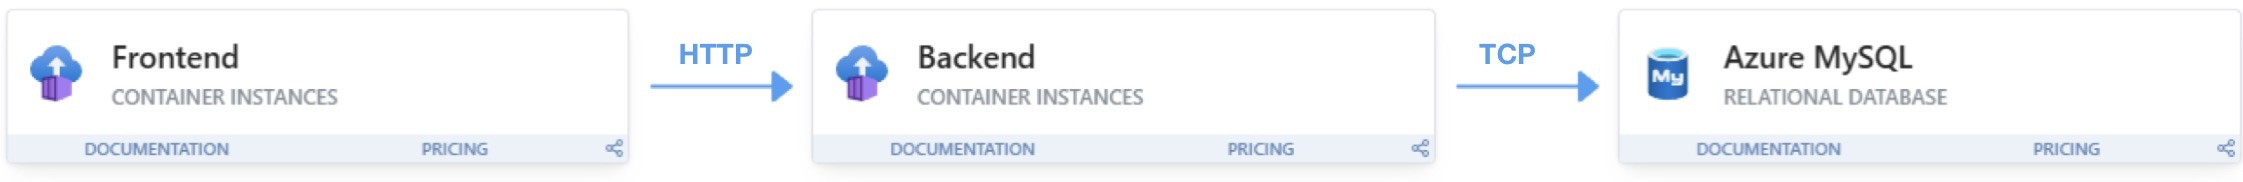
\includegraphics[width=1\linewidth]{img/diagrama_despliegue.png}
    \caption{Diagrama de Despliegue}
    \label{fig:diagrama_despliegue}
\end{figure}


\subsubsection{Componentes}
La aplicación desarrollada se encuentra desplegada en Azure, y consta de dos \textit{Azure Container Instances}, que ejecutan la parte cliente y la parte servidor mediante las imágenes de Docker publicadas en DockerHub. Adicionalmente, se usa una instancia de \textit{Azure Database for MySQL flexible server} para ejecutar la base de datos.

\subsubsection{Comunicación entre componentes}
La comunicación entre el Cliente (\textit{frontend}) y el Servidor (\textit{backend}) ocurre a través de HTTP. El cliente hace peticiones a los distintos \textit{endpoints} del servidor, y este responde con la información solicitada. Adicionalmente, el cliente tiene configurado un \textit{proxy}, ya que sin él las peticiones no llegarían al servidor. Este \textit{proxy} apunta a la dirección IP asignada al contenedor que contiene el \textit{backend}, por lo que si ese contenedor es eliminado y vuelto a crear, la IP del \textit{proxy} quedará obsoleta. Es por esto que el workflow de despliegue del servidor tiene un paso adicional en el que reinicia el contenedor del cliente. Esto asegura que el \textit{proxy} se configura apuntando al nuevo contenedor levantado, permitiendo que la comunicación fluya sin problemas. Es importante mencionar que este \textit{proxy} es un elemento interno de Angular, no es un servicio externo.

Por otro lado, la comunicación entre el servidor y la base de datos se realiza mediante el protocolo MySQL sobre TCP (puerto 3306) utilizando controladores JDBC. Azure expone la base de datos en una URL pública. Cuando se genera el contenedor del servidor, se le pasa esta URL como variable de entorno, para que la aplicación pueda usarla para conectar con la base de datos. De igual manera, las credenciales necesarias para la conexión también se pasan como variables de entorno.

\subsection{Modelo del dominio} 
El modelo de dominio identifica los distintos elementos existentes en el dominio de la aplicación, y los recoge en una serie de entidades con atributos y características, de forma que la aplicación pueda trabajar con ellos. En esta sección se detallan estas entidades, así como sus atributos y las relaciones entre ellas.

\subsubsection{Entidades}
Las entidades de la aplicación junto con sus atributos vienen recogidas en la siguiente tabla:

\begin{table}[h]
\small
\centering
\caption{Resumen de Entidades y sus Atributos}
\begin{tabularx}{\textwidth}{@{} l p{4cm} X @{}}
\toprule
\textbf{Entidad} & \textbf{Descripción} & \textbf{Atributos} \\ \midrule
\textbf{Usuario} & Personas que utilizan la aplicación. & Nombre de usuario, contraseña, nombre público, correo electrónico, murales miembros, roles. \\ \addlinespace
\textbf{Actividad} & Entrenamientos realizados por los usuarios. & Nombre, tipo, visibilidad, coordenadas, usuario propietario, ruta, resumen. \\ \addlinespace
\textbf{Ruta} & Actividades realizadas en un mismo circuito. & Nombre, descripción, distancia total, elevación ganada, coordenadas, visibilidad, creador. \\ \addlinespace
\textbf{Mural} & Grupos de usuarios para compartir contenido. & Nombre, descripción, código acceso, visibilidad, propietario, miembros, baneados, miniatura, cabecera. \\ \bottomrule
\end{tabularx}
\end{table}

\subsubsection{Objetos valor}
Además de las entidades, se han creado una serie de objetos auxiliares que reciben el nombre de "objetos valor". Estos son objetos sin identidad, cuya única función es facilitar la estructura, comunicación, o adherencia a reglas de negocio. Se identifican los siguientes objetos valor:

\begin{table}[h]
\small
\centering
\caption{Objetos valor del modelo del dominio}
\label{tab:objetos_valor}
\begin{tabularx}{\textwidth}{@{} l p{4.5cm} X @{}}
\toprule
\textbf{Objeto valor} & \textbf{Descripción} & \textbf{Atributos} \\ \midrule
\textbf{Coordinates} & Conjunto de coordenadas en el espacio. & Latitud, longitud. \\ \addlinespace
\textbf{ActivitySummary} & Métricas principales para evitar recalcular datos. & Tiempo inicio, distancia total, tiempo total, altura ganada, media por métrica, records. \\ \addlinespace
\textbf{Record} & Mapea un objetivo con el mejor desempeño obtenido. & Objetivo, marca. \\ \addlinespace
\textbf{Datapoint} & Información recogida por el hardware en un instante. & Hora, latitud, longitud, elevación, pulsaciones, cadencia, otros. \\ \bottomrule
\end{tabularx}
\end{table}


\subsection{API REST}
La comunicación con el servidor de la aplicación se realiza mediante una API REST. Todos los endpoint de la api empiezan por \texttt{/api/\{Entidad\}}, donde entidad corresponde a una de las entidades de la aplicación, en inglés: users, activities, routes, murals. La API trabaja con DTOs (Data Transfer Object), lo que le permite un mayor control sobre los datos enviados y recibidos. Por ejemplo, al devolver una ruta se puede enviar con todas las actividades que forman parte de ella, u omitiendo esa lista, de forma que la petición es más ligera.

Se puede consultar un listado de todos los recursos, sus DTOs y endpoints en el anexo \ref{anexo:api_rest}

\subsection{Arquitectura del servidor} 
Para asegurar que la aplicación funcione de manera eficiente y que, a futuro, sea fácil implementar cambios, es importante seguir una arquitectura clara a la hora de diseñar los distintos servicios. En el caso del servidor, se ha implementado una arquitectura por capas, dividiendo el servidor en tres capas principales, con otros paquetes trasversales. Las capas son las siguientes:
\begin{itemize}
    \item \textbf{Controlador:} es el punto de entrada al servidor, encargado de recibir peticiones HTTP y transformar los datos recibidos en objetos que el resto del \textit{backend} pueda entender. Asimismo, es el responsable de empaquetar los resultados que devuelven las siguientes capas en mensajes HTTP que puedan ser enviados como respuesta al cliente. 
    \item \textbf{Servicio:} esta capa contiene la lógica de negocio. Los controladores la usan para realizar las distintas operaciones solicitadas por los clientes. Se ocupa de comprobar permisos de usuarios y realizar operaciones sobre los objetos del sistema.  
    \item \textbf{Repositorio:} se ocupa de la conexión con la base de datos. Ofrece distintos métodos para obtener objetos de la base de datos, así como para actualizar los datos almacenados. 
\end{itemize}

La comunicación entre capas es estrictamente unidireccional. Objetos en la capa Controlador hacen uso de objetos en la capa Servicio, que a su vez hacen uso de objetos en la capa Repositorio. Objetos en una misma capa no se comunican entre sí, y no hay comunicación de una capa con la anterior. 

Además de estas capas principales, la arquitectura permite la existencia de algunos paquetes trasversales, que pueden ser usados en todas las capas. En este caso sólo se hace uso de un paquete trasversal, Modelo, que contiene las representaciones de las distintas entidades identificadas en el dominio.

La figura \ref{fig:arq_servidor} resume las capas, sus objetos, y las relaciones entre ellos:
\begin{figure}[H]
    \centering
    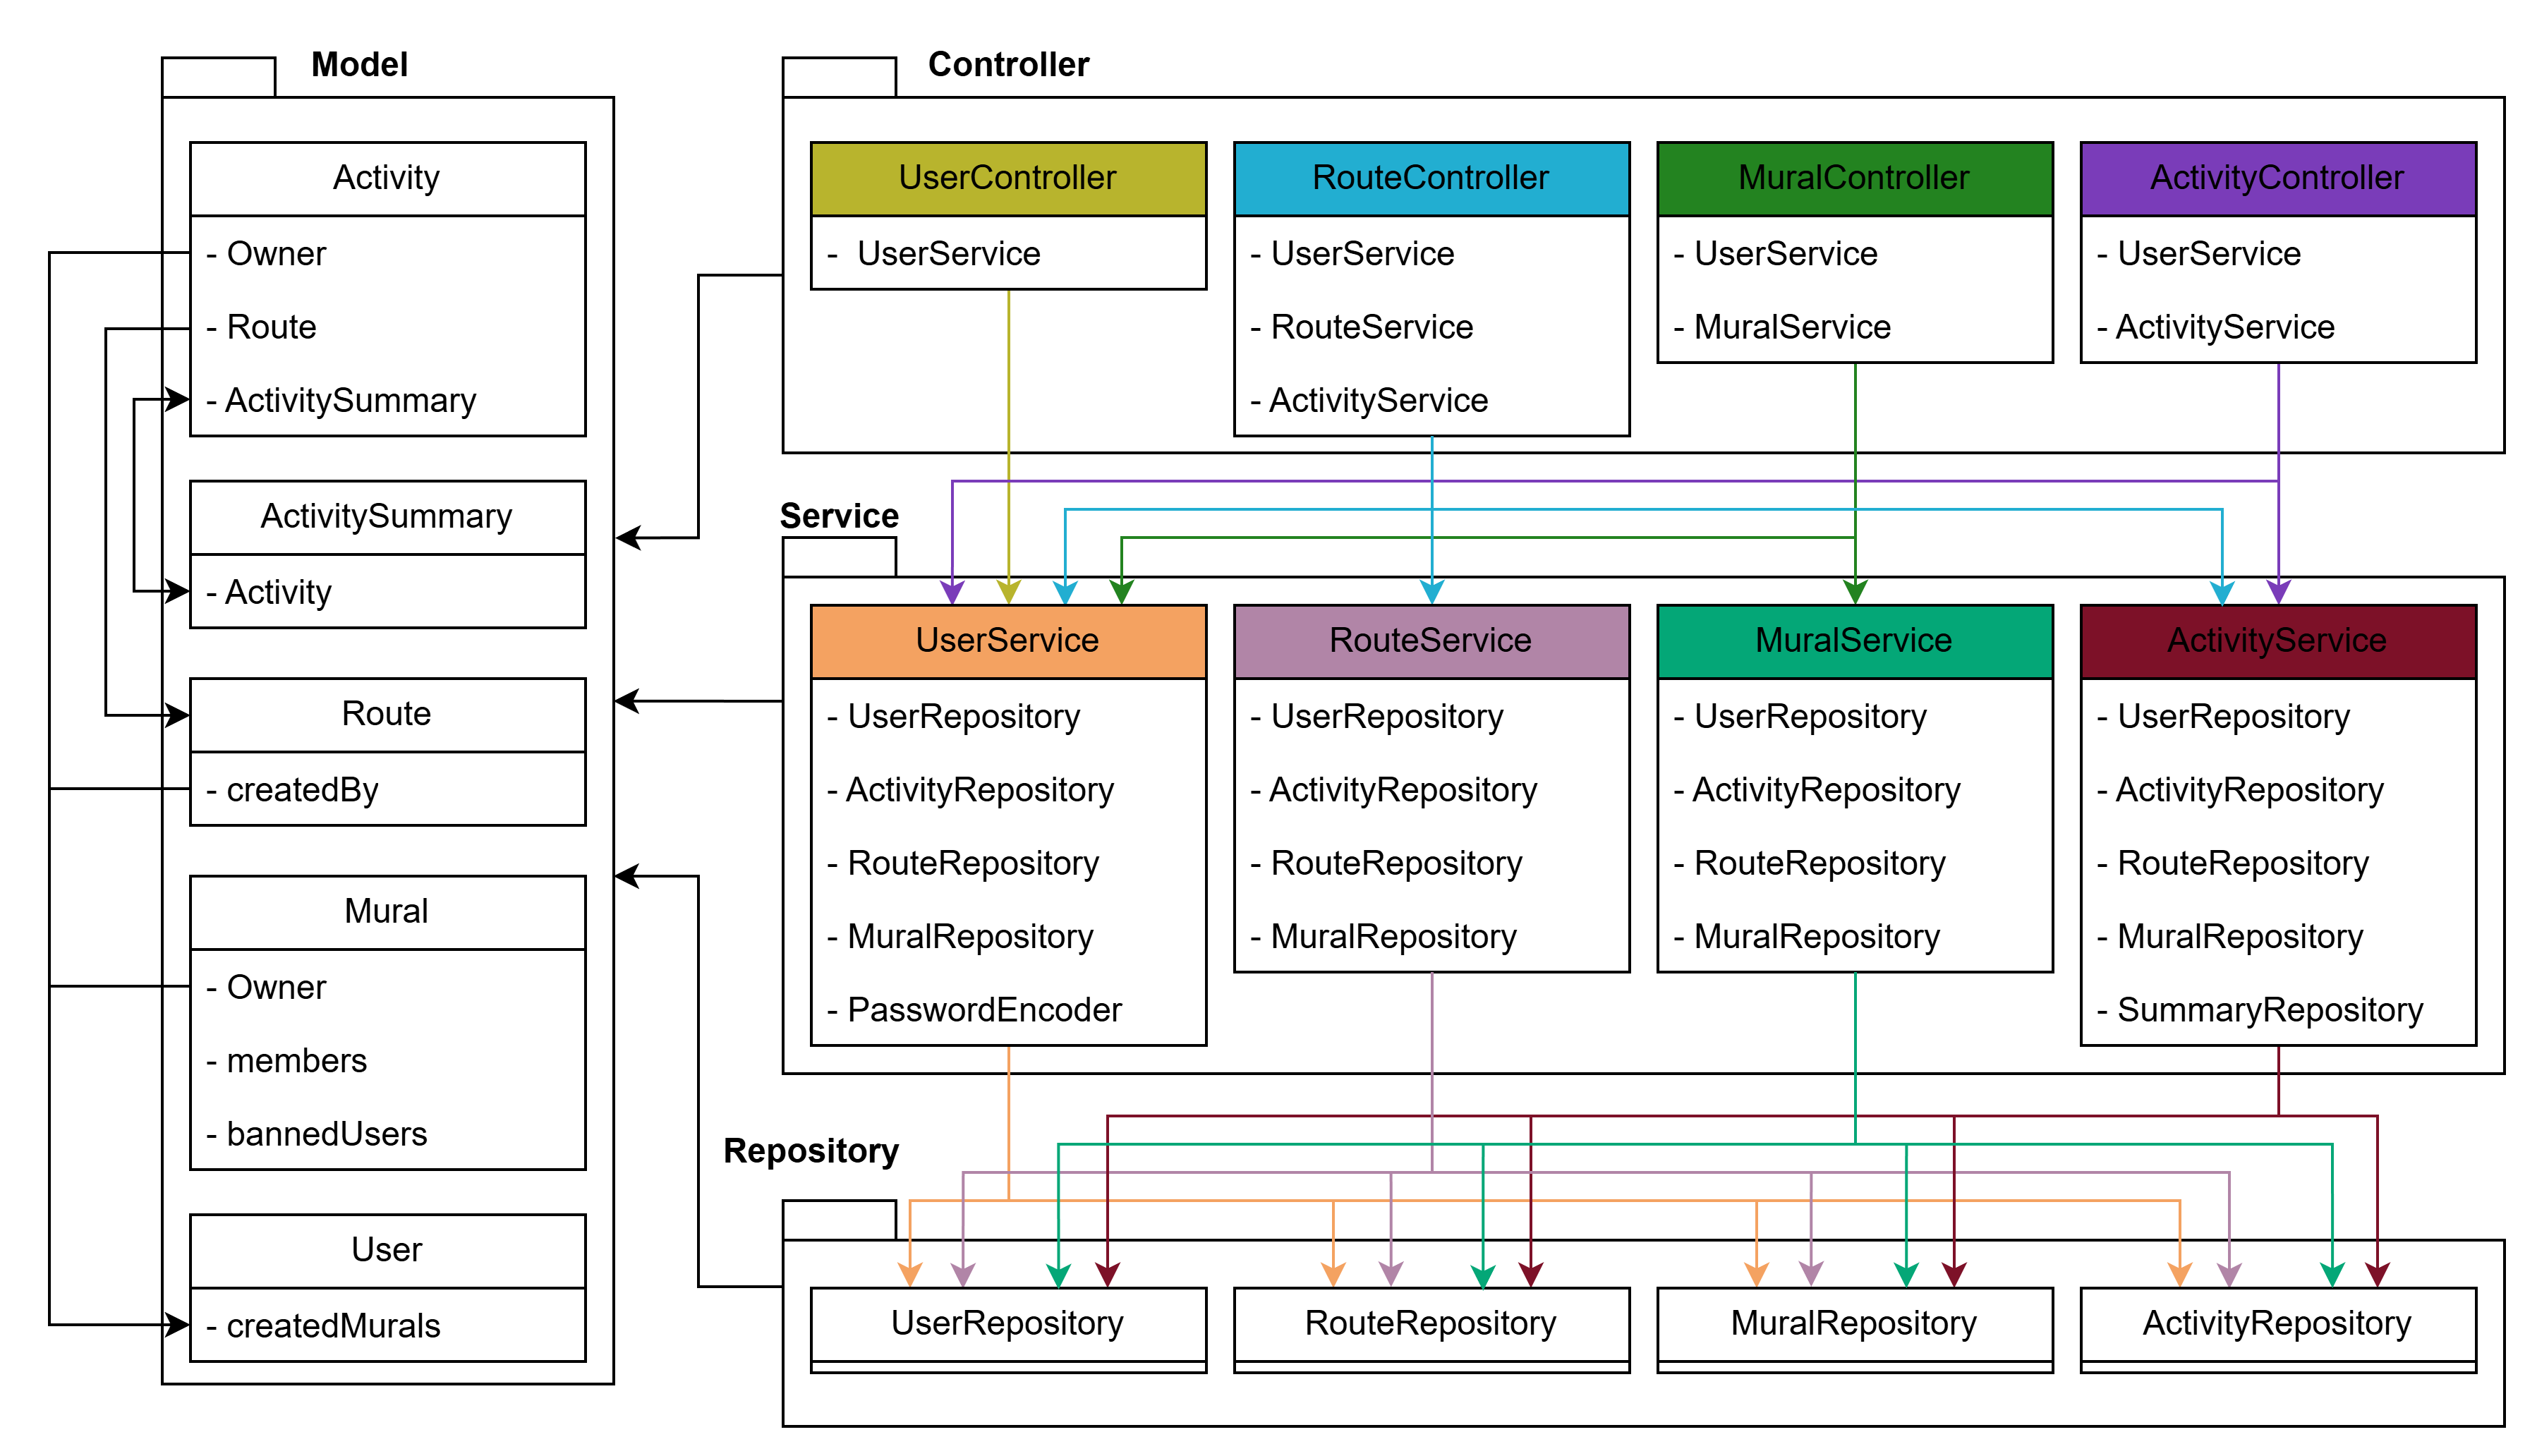
\includegraphics[width=0.75\linewidth]{img/arq_servidor.png}
    \caption{Diagrama de clases mostrando las capas del servidor y las relaciones entre controladores, servicios, y repositorios}
    \label{fig:arq_servidor}
\end{figure}

\noindent El diagrama muestra una versión simplificada de la realidad, para mantener la claridad visual. Concretamente, se han llevado a cabo las siguientes simplificaciones:
\begin{itemize}
    \item No se muestran la mayoría de atributos de cada clase. Sólo se representan en el diagrama aquellos atributos que enlazan con otro objeto representado, y algún servicio auxiliar adicional como el \texttt{PasswordEncoder}.
    \item No se muestran las relaciones de cada controlador, servicio, y repositorio con cada clase del paquete modelo. El objetivo de este diagrama es mostrar la arquitectura en capas y el flujo lineal de dependencias entre las capas de controlador, servicio, y repositorio. Como tal, se ha preferido no incluir las relaciones independientes de cada clase con los modelos, ya que añadiría contenido innecesario. En vez de eso, se indica que todas las capas usan las clases del paquete, sin entrar en detalle.
\end{itemize}

\subsection{Arquitectura del cliente} 
De igual manera que en el servidor, también es importante mantener una arquitectura bien definida en el cliente. En este caso, también se hace uso de una arquitectura por capas, aunque es más laxa que en el servidor. Se divide el código en tres módulos principales:
\begin{itemize}
    \item \textbf{Componente:} es el punto de contacto con el usuario. Sus responsabilidades incluyen generar las vistas, registrar las acciones del usuario, almacenar datos a corto plazo y realizar algunos cálculos sencillos.
    \item \textbf{Servicio:} es el punto de contacto con el servidor. Sus responsabilidades incluyen la comunicación con el servidor, la realización de operaciones y cálculos, y el almacenamiento de variables e información que debe persistir más allá del ciclo de vida de un componente (función caché).
    \item \textbf{Modelo:} se encarga de ofrecer una representación de las entidades del dominio. Contiene una serie de \textit{Data Transfer Objects} (DTO) usados para comunicación con el servidor, junto con las clases completas que se utilizan para cachear o realizar cálculos.
\end{itemize}

La comunicación entre estos módulos sigue un flujo determinado, ilustrado en la figura \ref{fig:arq_cliente_vision_general}.

\begin{figure}[H]
    \centering
    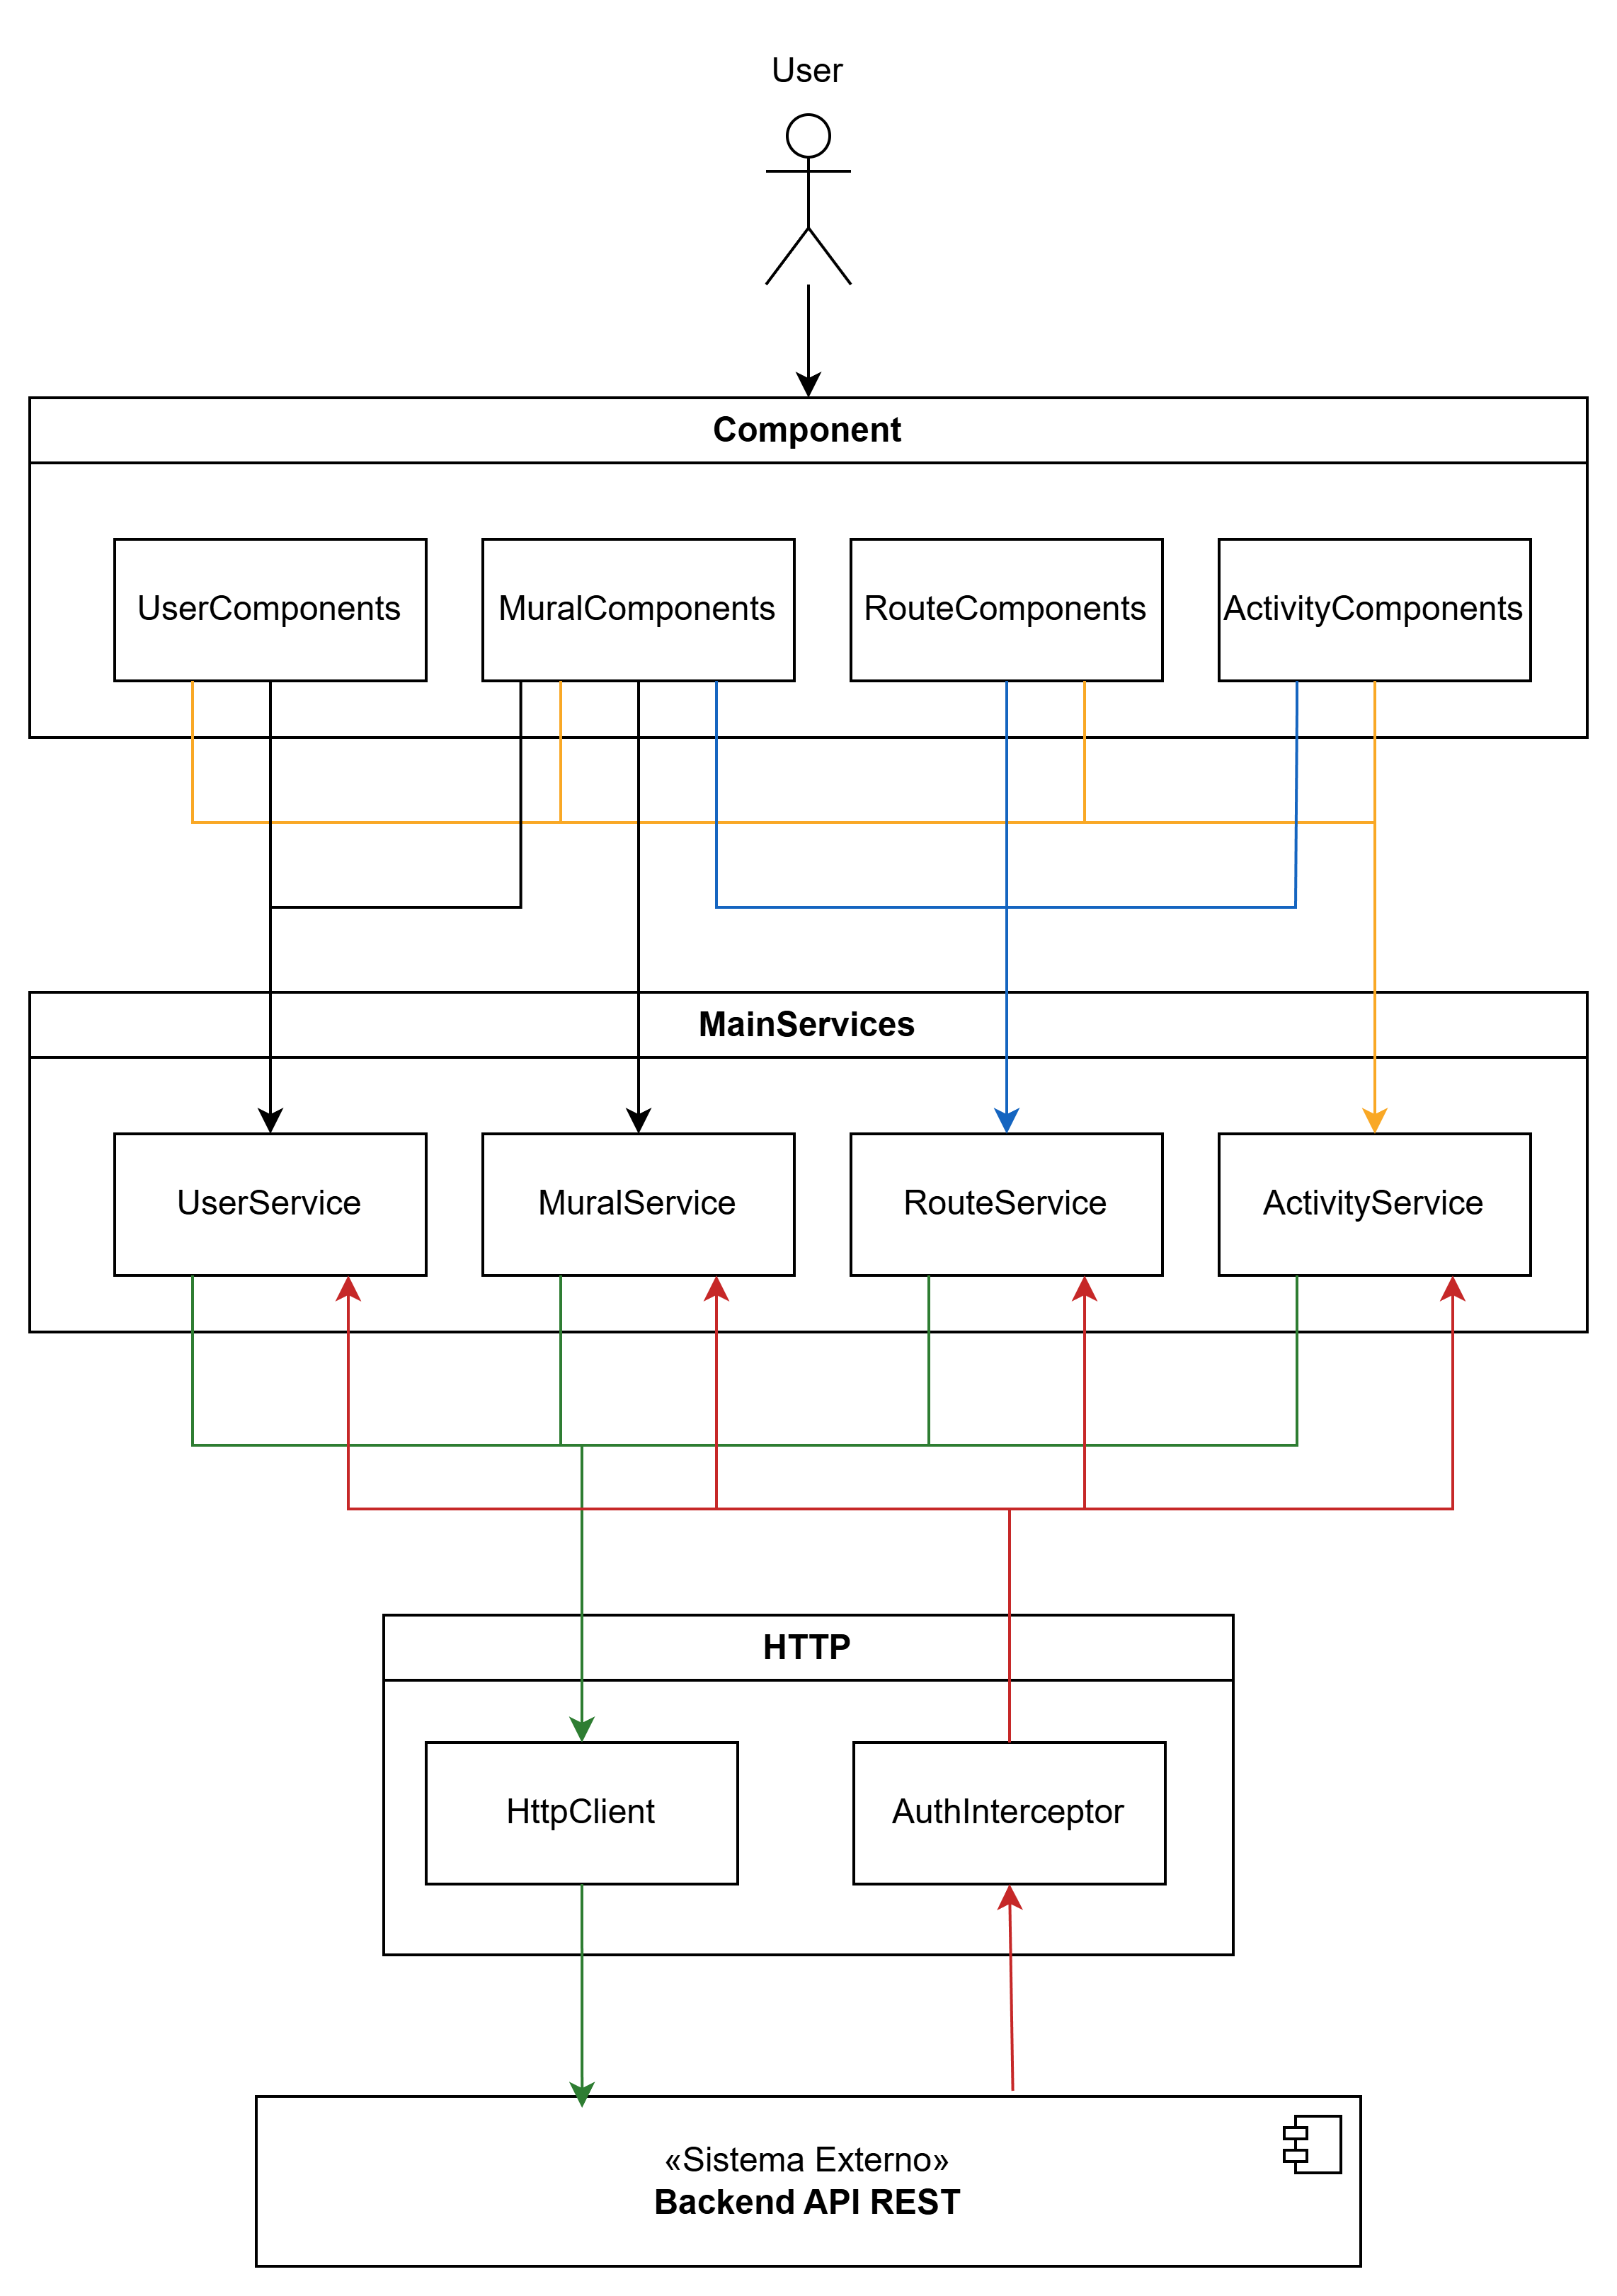
\includegraphics[width=0.4\linewidth]{img/arq_cliente_vision_general.png}
    \caption{Arquitectura del cliente - Visión general}
    \label{fig:arq_cliente_vision_general}
\end{figure}

El usuario interactúa con los componentes de Angular, que transmiten las acciones a los servicios principales, los cuales realizan operaciones o envían peticiones al servidor a través de un HttpClient. Cuando el servidor responde, la respuesta es leída primero por un AuthInterceptor. Si la respuesta tiene código de error, el interceptor lo gestiona, por norma general mostrando un mensaje. Cuando las respuestas son exitosas las deja pasar como si no existiera. Durante todo este flujo, ambos módulos utilizan objetos del módulo Model, y aprovechan funcionalidades de una serie de servicios auxiliares. Estas relaciones se pueden consultar en las figuras \ref{fig:arq_cliente_componentes} y \ref{fig:arq_cliente_servicios}. 

\begin{figure}[H]
    \centering
    \begin{minipage}{0.48\linewidth}
        \centering
        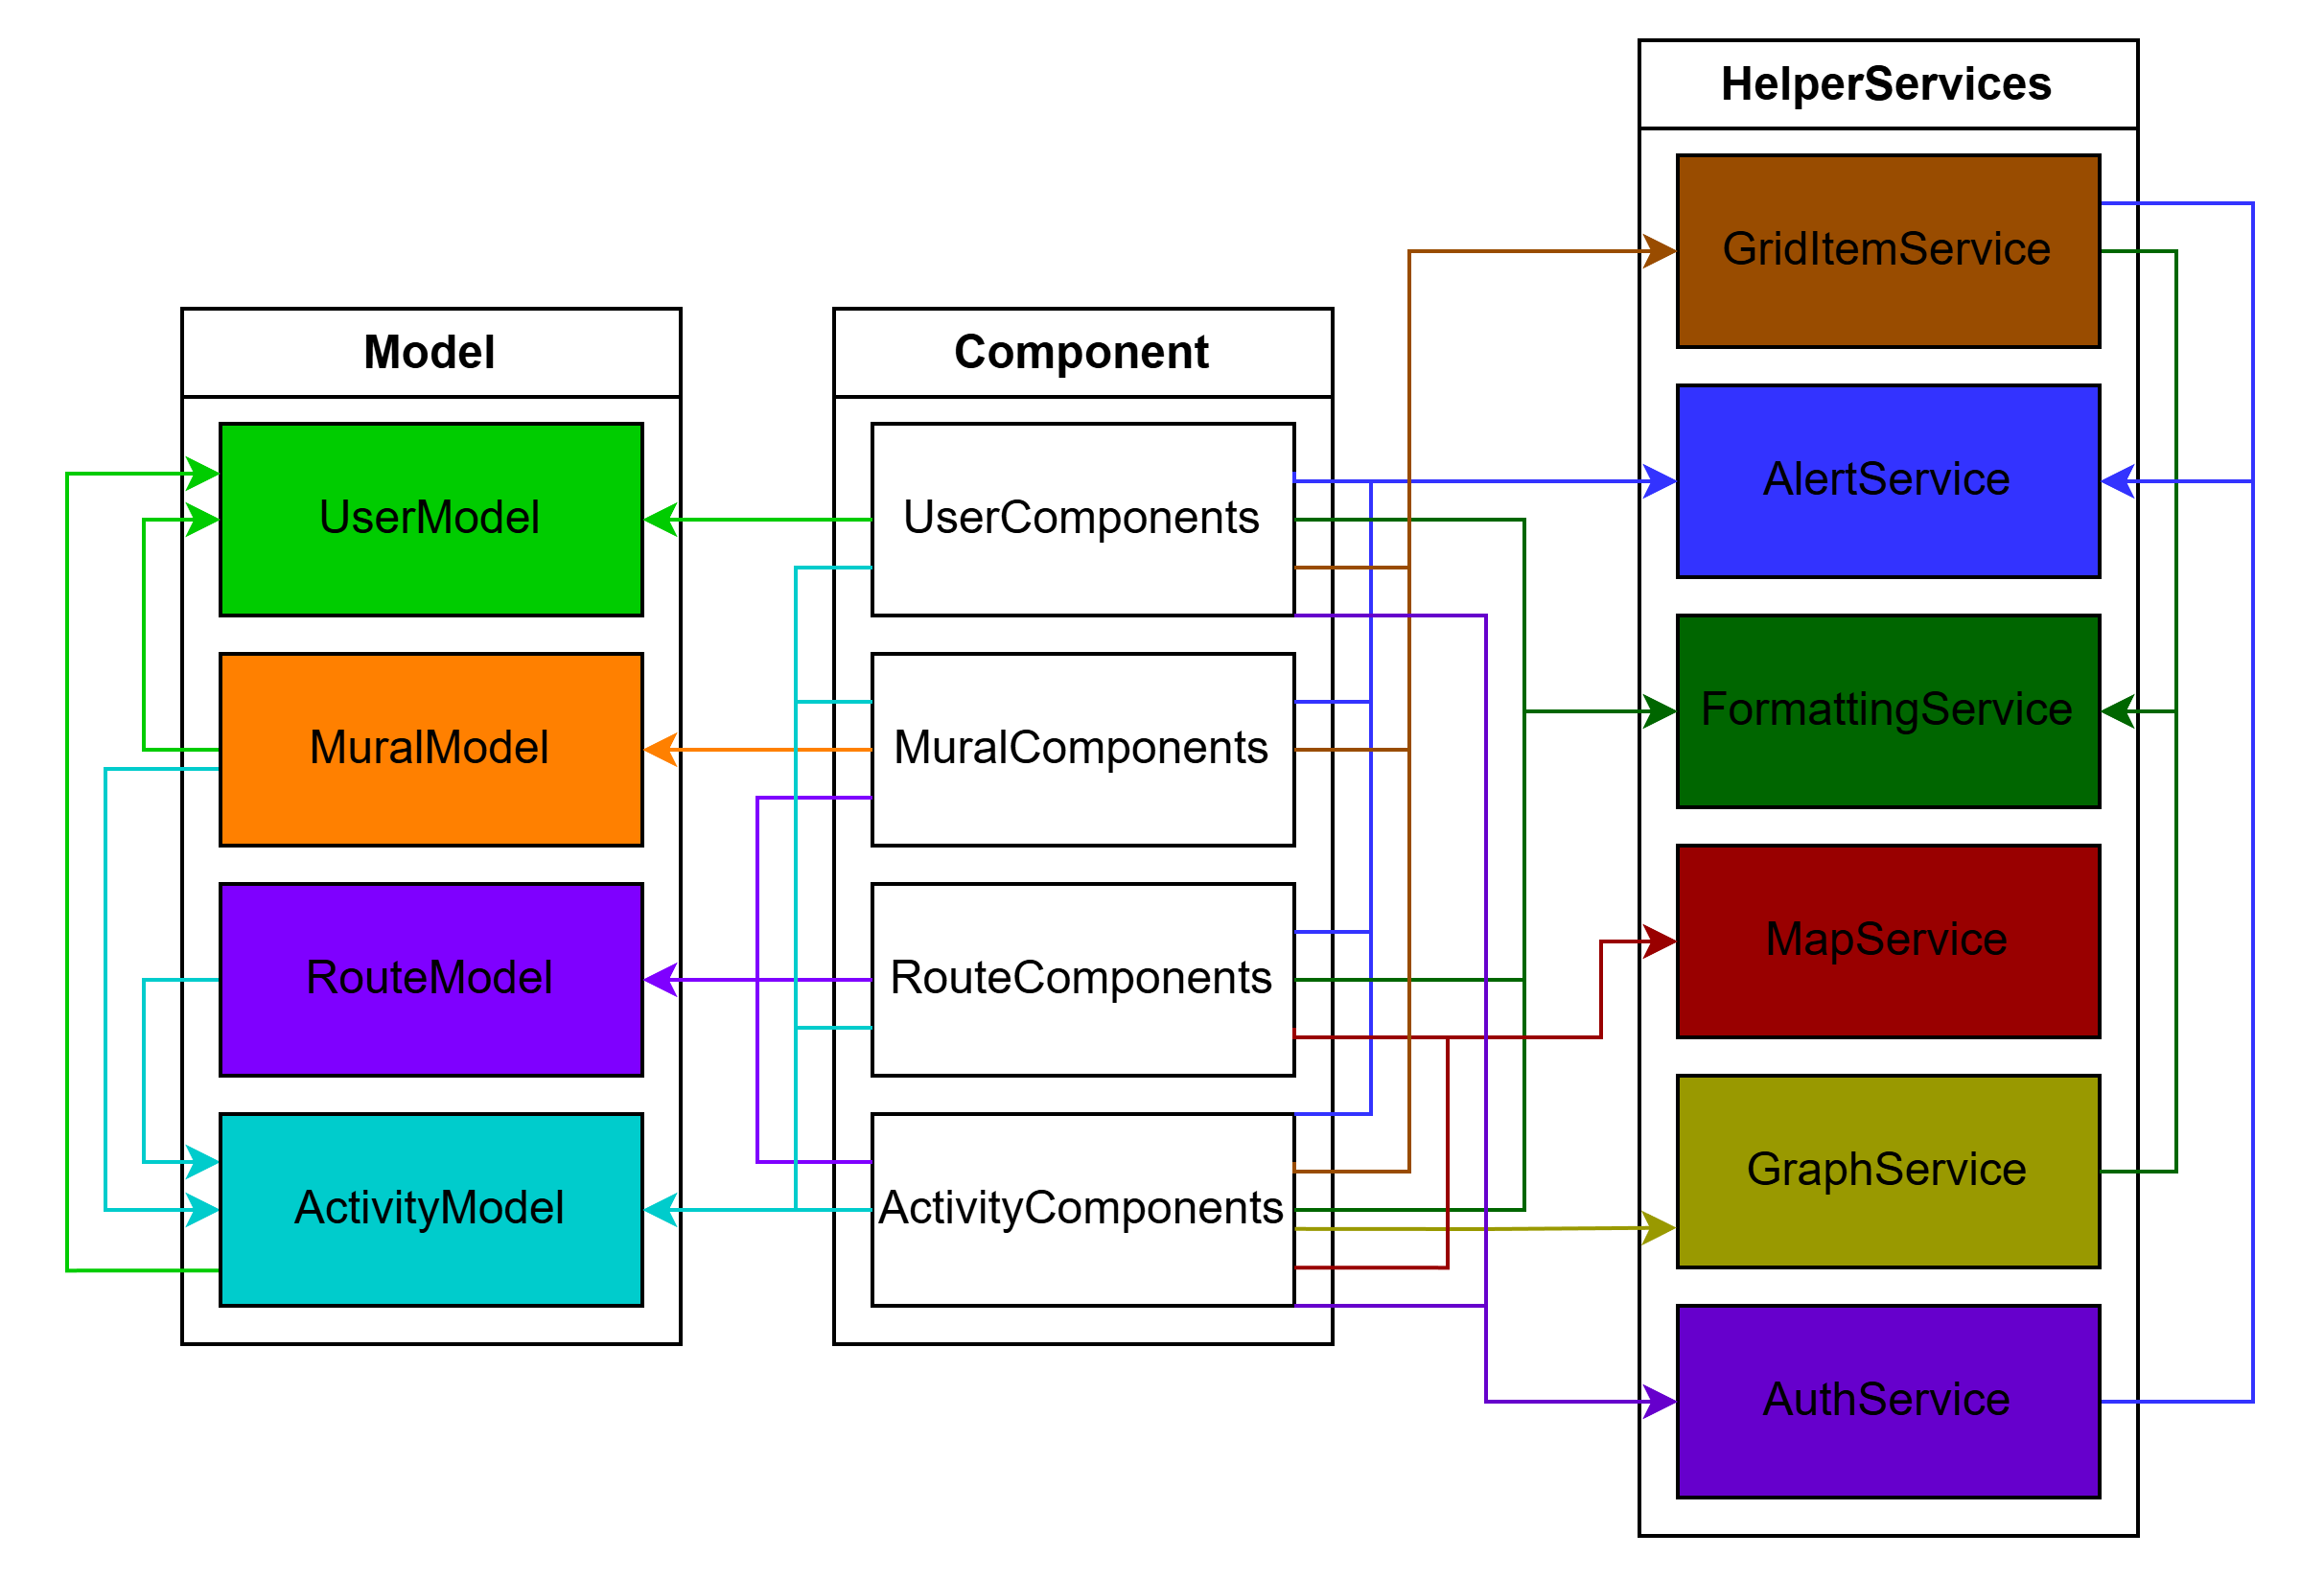
\includegraphics[width=\linewidth]{img/arq_cliente_componentes.png}
        \caption{Arquitectura del cliente - Uso de Modelos y Servicios Auxiliares por Componentes}
        \label{fig:arq_cliente_componentes}
    \end{minipage}
    \hfill
    \begin{minipage}{0.48\linewidth}
        \centering
        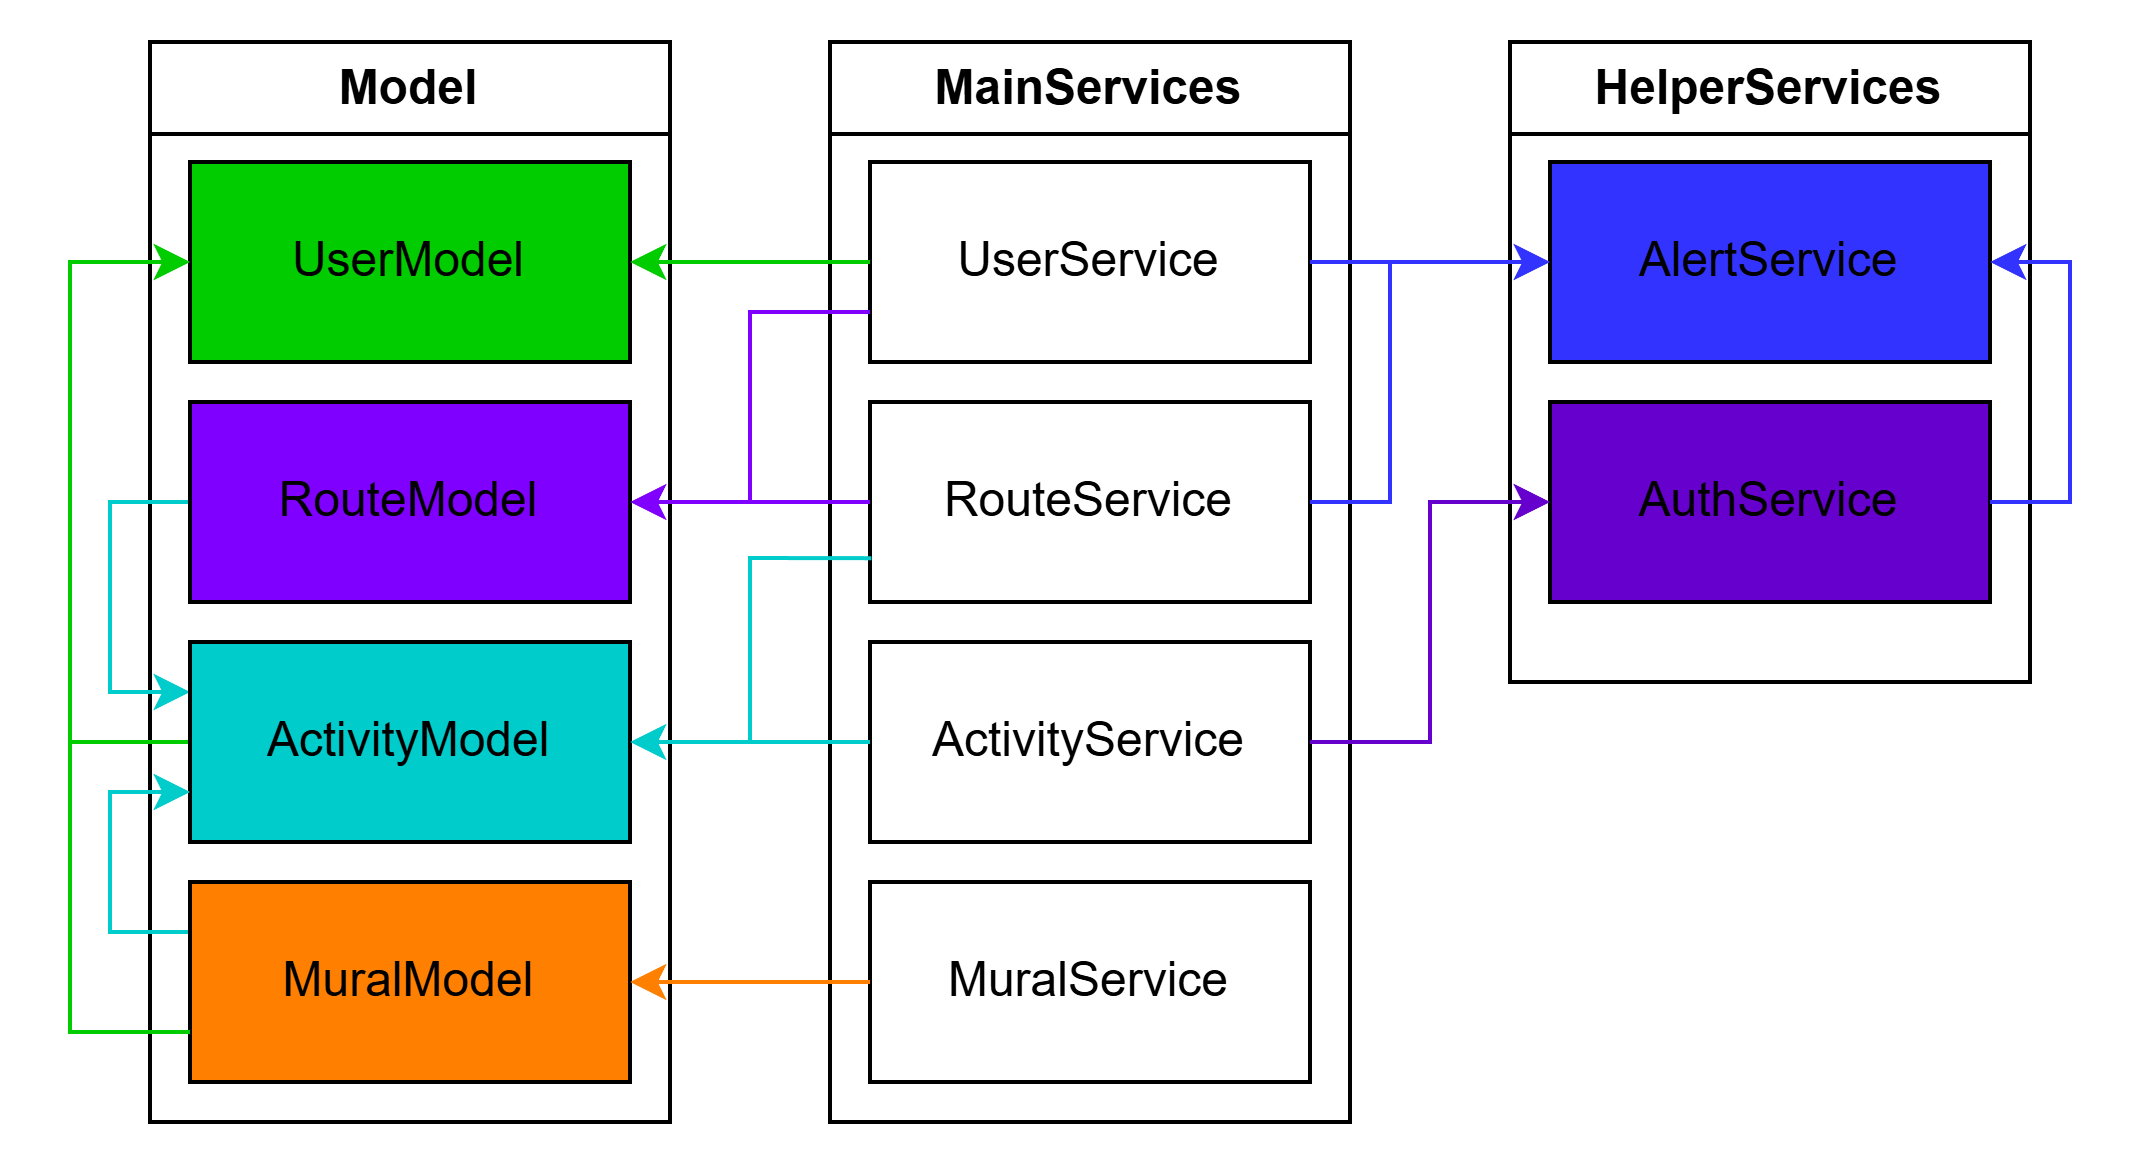
\includegraphics[width=\linewidth]{img/arq_cliente_servicios.png}
        \caption{Arquitectura del cliente - Uso de Modelos y Servicios Auxiliares por Servicios principales}
        \label{fig:arq_cliente_servicios}
    \end{minipage}
\end{figure}

Los diagramas presentados muestran una representación simplificada de la arquitectura real. El proyecto contiene más componentes de los que se muestran en estos diagramas. Sin embargo, para mejorar la claridad visual de los diagramas, se ha decidido agrupar los componentes existentes en bloques funcionales. De igual manera, existen algunos modelos y servicios auxiliares en la arquitectura real que no están siendo representados en los diagramas.

\section{Implementación} 
La implementación de la aplicación ha sido la parte que más tiempo y esfuerzo ha requerido, y durante el proceso han surgido una serie de problemas, errores, y decisiones que han necesitado resolución. Esta sección describe los aspectos de la implementación más destacables, así como los distintos problemas que han surgido durante el proceso y cómo se han solucionado.

\subsection{Visibilidad}
Dada la naturaleza social de la aplicación, es necesario determinar cómo se va a gestionar la visibilidad de las distintas entidades. Se debe respetar la privacidad de los usuarios, por lo que no pueden ser todos los recursos creados públicos. Por otro lado, tampoco pueden ser todos privados, pues entonces no tendría sentido que convivieran varios usuarios en la aplicación. Así pues, es necesario permitir a los usuarios gestionar la visibilidad de sus recursos. 

Para que los usuarios puedan personalizar adecuadamente la visibilidad de sus recursos, se plantean las siguientes visibilidades:
\begin{itemize}
    \item \textbf{\texttt{PUBLIC}:} recursos con visibilidad pública son accesibles por todos los usuarios y murales. Cualquiera que haga una petición a /api/recurso/id podrá visualizar su información.
    \item \textbf{\texttt{MURAL\_PUBLIC}:} recursos con esta visibilidad son visibles para cualquier mural en el que esté el usuario propietario/creador del recurso.
    \item \textbf{\texttt{MURAL\_PRIVATE}:} recursos con esta visibilidad son visibles para un conjunto concreto de murales seleccionados por el propietario, siempre que sea miembro de ellos.
    \item \textbf{\texttt{PRIVATE}:} recursos con visibilidad privada sólo son visibles para el usuario propietario.
\end{itemize}

Si un mural tiene visibilidad de un recurso determinado, todos sus miembros obtienen visibilidad del recurso a través de ese mural. Es decir, si al pedir el recurso especifican que realizan la petición como miembro del mural, podrán visualizarla. Sin embargo, si realizan la petición de manera normal, no tendrán visibilidad del recurso. Si el usuario abandona el mural por cualquier razón, pierde visibilidad de los recursos que le exponía ese mural.

Los recursos con visibilidad son Actividades, Rutas, y Murales. Sin embargo, no todos estos recursos tienen las mismas visibilidades. Concretamente, los Murales sólo pueden ser \texttt{PUBLIC} o \texttt{PRIVATE}, mientras que las Rutas tienen esas visibilidades junto con \texttt{MURAL\_PUBLIC}, y las Actividades son los únicos recursos que hacen uso de todos los posibles valores de visibilidad. 

La visibilidad se implementa en la aplicación mediante un enumerado \texttt{VisibilityType}, y una clase \texttt{Visibility}. La clase \texttt{Visibility} tiene dos atributos: una instancia de \texttt{VisibilityType}, y una lista de murales permitidos, que sólo entra en juego cuando la visibilidad es \texttt{MURAL\_PRIVATE}.

La principal dificultad en la implementación de las visibilidades viene de la gestión de las rutas, dado que tener visibilidad de una ruta te permite añadir actividades a la misma. Si luego el creador de la ruta quiere reducir su visibilidad o eliminarla, se debe gestionar lo que debe ocurrir en estos casos. Se han considerado varias opciones:
\begin{enumerate}
    \item Borrar la ruta de las actividades que la contengan.
    \begin{itemize}
        \item Ventajas: se elimina completamente la información de la ruta. Si ha sido eliminada por temas de privacidad, esta solución evita problemas.
        \item Desventajas: perjudica a los usuarios que estuvieran usando la ruta, pues las actividades asignadas a esta ruta quedan sin ruta y se pierde su agrupación.
    \end{itemize}
    \item Borrar la ruta creada por el usuario y crear una copia para el uso del resto de usuarios.
    \begin{itemize}
        \item Ventajas: Se mantiene la agrupación de las actividades de otros usuarios.
        \item Desventajas: quita parte de la agencia de los usuarios sobre la información contenida en rutas creadas, pues al crear una copia, la información de la ruta no es eliminada.
    \end{itemize}
    \item Bloquear la eliminación de la ruta hasta que nadie la esté usando.
        \begin{itemize}
        \item Ventajas: cuando un usuario borra una ruta se elimina toda la información que se generó al crearla, sin perjudicar al resto de usuarios.
        \item Desventajas: quita parte de la agencia del usuario sobre su propia información, ya que hace que dependa de la acción de otros usuarios para poder eliminarla. Además, si no se ofrece una forma de comunicar a los otros usuarios que deben dejar de usar la ruta, podría quedarse en este estado de manera indefinida.
    \end{itemize}
\end{enumerate}

Se ha tomado la decisión de implementar la opción tercera como solución inicial, planteando a futuro la implementación de la solución segunda, permitiendo al propietario de la ruta decidir entre una u otra. 

Esta decisión busca asegurar que los usuarios que usan una ruta no pierdan la asociación entre sus actividades por decisión de otro usuario, asegurando a la vez el borrado real de los datos, en vez de su sustitución por otros.

\subsection{Gestión de caches}
Otro aspecto que aporta cierta complejidad es la gestión de cachés en el cliente. Es decir, el almacenado de ciertos valores que son necesitados frecuentemente durante un periodo corto de tiempo, para poder acceder a ellos sin que sea necesario contactar con el servidor.

Originalmente, los datos obtenidos por un componente sólo eran necesarios en ese componente. Sin embargo, según la aplicación se desarrolló más a fondo y se fueron creando componentes más específicos, surgió la necesidad de compartir información entre varios componentes. La estrategia anterior de que cada componente haga una petición separada es ineficiente, pues se repiten peticiones y se malgasta memoria. Tampoco es apropiado designar a un componente como propietario de los datos, ya que al cambiar a otro componente el propietario a menudo es destruido automáticamente por Angular, y sus datos se pierden. Así, se tomó la decisión de, en casos donde varios componentes necesiten acceder a los mismos datos, almacenarlos en servicios que hacen las veces de \textit{cachés}. La implementación de estas \textit{cachés} ha sido mediante la clase \texttt{BehaviorSubject}, una clase de la librería reactiva de Angular que implementa el patrón \texttt{Observer}, almacenando un valor y permitiendo a suscriptores recibir actualizaciones al mismo de manera asíncrona, o bien leer el valor actual del mismo.

\subsection{Interceptores y manejo de errores}
El manejo de errores es algo esencial en toda aplicación software, y esta no es excepción. Sin embargo, el alcance de la mayoría de proyectos desarrollados en la universidad no cubre a fondo el manejo de errores, por lo que se ha presentado como un obstáculo y oportunidad de aprendizaje.

\noindent Para centralizar el manejo de errores se han tomado las siguientes medidas:
\begin{itemize}
    \item En el servidor, se ha implementado una clase \texttt{CustomExceptionHandler} anotada con \texttt{@RestControllerAdvice}, conteniendo métodos anotados con \texttt{@ExceptionHandler(ExcepcionPersonalizada.class)}. Esta clase y métodos se encargan de, cuando se lancen errores de las clases especificadas, reaccionar de la manera especificada en el método correspondiente. Estos métodos traducen los errores lanzados por los servicios, como \texttt{EntityNotFoundException}, en códigos de error HTTP, como 404, y posteriormente devuelven una respuesta con el código de error correspondiente, junto con el mensaje especificado en la excepción (si lo hubiera), o un mensaje predeterminado para cada código.
    \item En el cliente, se ha implementado un auth-interceptor.service, con un método intercept, que lee todas las respuestas del servidor. Deja pasar sin modificaciones las respuestas correctas, pero cuando lee respuestas erróneas las intercepta, mostrando el mensaje de error correspondiente.
\end{itemize}
De nuevo, estas soluciones son estándar en aplicaciones software, pero se consideran dignas de mención dado que es la primera vez que el autor necesita enfrentarse a estas situaciones, y han ofrecido una oportunidad de aprender de manera orgánica.

\subsection{Mapas}
La representación de las rutas y actividades en mapas era uno de los grandes interrogantes previos a la implementación de la aplicación, al ser una tecnología desconocida para el autor, y dado que no ha trabajado con tecnologías similares anteriormente.

Sin embargo, al contrario de las preocupaciones iniciales, ha resultado ser un proceso relativamente sencillo. La implementación de mapas simples mostrando una ruta o actividad ha resultado no ser un obstáculo muy grande, por lo que se planteó la posibilidad de utilizar mapas de manera más dinámica. Por ejemplo, en la página de selección de actividad, se ha implementado un \textit{popover} que muestra, en tamaño reducido, un mapa con el trazo de la actividad sobre la que se ubique el cursor. La implementación de esta funcionalidad sí ha implicado más dificultad técnica, debido principalmente a la naturaleza efímera de los \textit{popovers}. Dado que el contenedor sobre el que se colocará el mapa no existe en el momento de crear el componente de Angular, sino que se crea dinámicamente durante el flujo de vida del componente, ha sido necesario modificar la configuración de los mapas para que ocurra una vez el \textit{popover} ha sido creado, en vez de inmediatamente después de crear el componente.

Ese mismo problema también se ha mostrado en los mapas normales, y especialmente en los mapas mostrados al comparar actividades. En ambos casos los mapas se encuentran en una sección que permite navegación por pestañas. Esto significa que, al cambiar de pestaña, el contenedor del mapa deja de existir, lo cual causa problemas. Lo mismo ocurre en la comparación de actividades, ya que permite mostrar un número variable de mapas. Esta gestión de varios contenedores de mapas, junto con su creación y eliminación dinámica han ofrecido retos particulares.

La solución a estos problemas ha sido crear un servicio auxiliar específico para la gestión de los mapas. Este servicio ofrece un método que permite crear un mapa dentro de un elemento HTML recibido como parámetro o identificado por su id. Así, cada vez que sea necesario un mapa, éste se crea desde cero, evitando los problemas que surgen de intentar usar un mapa que ya no existe.

\subsection{Visualización de gráficos}

Otro problema que surgió durante el desarrollo de la aplicación está relacionado con la librería de visualización de gráficos seleccionada. Durante el desarrollo se evaluaron varias opciones, entre ellas ApexCharts, D3.js y ngx-charts. Finalmente se optó por ngx-charts, debido a su enfoque Angular-first, su integración sencilla con el framework y el catálogo de gráficos que ofrece.

Sin embargo, esta librería introdujo ciertas dificultades, debido a que la forma en que dibuja gráficos de líneas con varias series no se adapta bien a los datos disponibles. El problema surge porque la librería recibe los datos como una serie de tuplas (parejas) de la forma \texttt{(x,y)}, donde \texttt{x} es una cadena de caracteres, e \texttt{y} es un número. Debido a esto, no es capaz de interpolar el valor de y para un valor de \texttt{x} inexistente, por lo que si recibe varias series que tienen distintos valores de \texttt{x} en un mismo rango, los muestra de forma errónea. Su comportamiento parece ser el siguiente:
\begin{enumerate}
    \item Coloca parejas de valores \texttt{(x,y)} al principio y en orden cuando todas las series tienen una pareja con el valor de \texttt{x} específico
    \item A continuación, coloca aquellas parejas de valores cuyo \texttt{x} no tenga un valor de \texttt{y} asociado en todas las series
\end{enumerate}
Esto lleva a situaciones donde, con las series \{1,2,6,9,10\}, y \{1,2,3,6,9\}, muestra los valores del eje \texttt{x} en el siguiente orden \{1,2,6,9,10,3\}, en vez de el esperado \{1,2,3,6,9,10\}. Se puede experimentar con la librería  en \href{https://stackblitz.com/edit/swimlane-line-chart}{\uline{stackblitz}}\footnote{\url{https://stackblitz.com/edit/swimlane-line-chart}} para ver su comportamiento exacto. La figura \ref{fig:ngx_charts_wrong} muestra la gráfica generada con los valores propuestos en el ejemplo.

\begin{figure}[H]
    \centering
    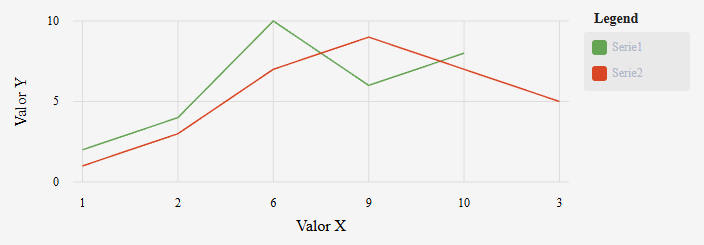
\includegraphics[width=0.75\linewidth]{img/ngx_charts_ejemplo_malo.png}
    \caption{Ejemplo del comportamiento inesperado de ngx-charts}
    \label{fig:ngx_charts_wrong}
\end{figure}

Para solucionar este problema ha sido necesario implementar un algoritmo que interpole los valores necesarios para asegurar que todas las series tengan los mismos valores de \texttt{x}.

Es un algoritmo iterativo que busca asegurar que todas las series tengan el mismo número de entradas y que usen los mismos valores de \texttt{x} en intervalos compartidos. A continuación se presenta una explicación del algoritmo. Para que sea más fácil de entender, se asumirá que el eje \texttt{x} representa distancia.
\begin{enumerate}
    \item Almacena en una variable todos los valores de \texttt{x} presentes entre todas las series, ordenados de menor a mayor.
    \item Ordena las series según el valor \texttt{x} de su último punto (en orden ascendiente de distancia total).
    \item Establece 0 como el punto inicial.
    \item Selecciona la serie en primera posición de la lista ordenada de series.
    \item Establece el final de la serie como punto final.
    \item Para cada serie a partir de la seleccionada, itera por todos los valores de \texttt{x} entre el punto inicial y el punto final, y:
        \begin{itemize}
            \item crea una lista vacía
            \item si la serie tiene un punto con ese valor de \texttt{x}, lo añade a la lista
            \item si la serie no contiene un punto con ese valor de \texttt{x}, calcula una estimación del valor esperado mediante interpolación lineal y lo añade a la lista
            \item si ha iterado por todos los puntos, actualiza la serie con los valores de la lista, y continúa con la siguiente serie
        \end{itemize}
    \item cuando ha tramitado todas las series, establece el punto final como punto inicial para la siguiente iteración.
    \item Si sólo queda una serie por seleccionar en la lista, el algoritmo acaba. Si no, vuelve al paso 4, seleccionando la siguiente serie en la lista.    
\end{enumerate}
Además, también elimina duplicados dentro de una serie. Por la naturaleza de los datos y cómo son tratados por las aplicaciones que los capturan o exportan, algunas series tienen valores de \texttt{x} repetidos. El algoritmo detecta estos casos y permite, o bien quedarse con el primer valor encontrado, o bien utilizar una media acumulada calculada a partir de todos los valores de \texttt{y} con ese valor de \texttt{x}.

Dos puntos destacan dentro del desarrollo del algoritmo, afines a la dificultad inherente al mismo. El primero es un error que surgió debido a una ordenación incorrecta de las series en el paso 2. Inicialmente, la ordenación de las series era en función de la cantidad de elementos en cada serie. Este sería un buen criterio si tenemos la certeza de que las series toman valores en intervalos fijos, sin valores duplicados ni saltos. Sin embargo, debido a la naturaleza de los datos, esto no se cumple. Por tanto, en ocasiones donde actividades más cortas tuvieran más puntos que una actividad más larga, el algoritmo fallaba. Debido a que el fallo viene de un supuesto incorrecto, fue difícil de identificar, aunque una vez identificado no fue complejo de solucionar.

El segundo es la identificación de duplicados y el cálculo de la media acumulada. Igual que el algoritmo de interpolación, la media se calcula mediante un algoritmo, si bien es mucho más sencillo. A continuación se detalla este proceso:
\begin{enumerate}
    \item Se identifica un duplicado cuando el nuevo elemento seleccionado de la serie con la que se está trabajando coincide con el último elemento añadido a la lista actualizada
    \item En este momento, si está activada la funcionalidad, se calcula una media utilizando el valor guardado en la lista y el valor actual. Esta media se calcula multiplicando el valor almacenado por un peso, correspondiente al número de duplicados encontrados hasta ahora, sin contar el actual. Luego se le suma el valor actual, y se divide entre el total de duplicados encontrados.
    \item se suma 1 al peso para que refleje el duplicado recién encontrado, y se continúa con el siguiente valor.
    \begin{itemize}
        \item Si el siguiente valor también es duplicado, repite el paso 2.
        \item Si el siguiente valor no es duplicado, restablece el peso a su valor inicial (1), y el algoritmo continúa con los siguientes valores.
    \end{itemize}
\end{enumerate}

La figura \ref{fig:ngx_algo_bad} muestra una selección de actividades en las que se puede ver el efecto del error de ordenación.
\begin{figure}[H]
    \centering
    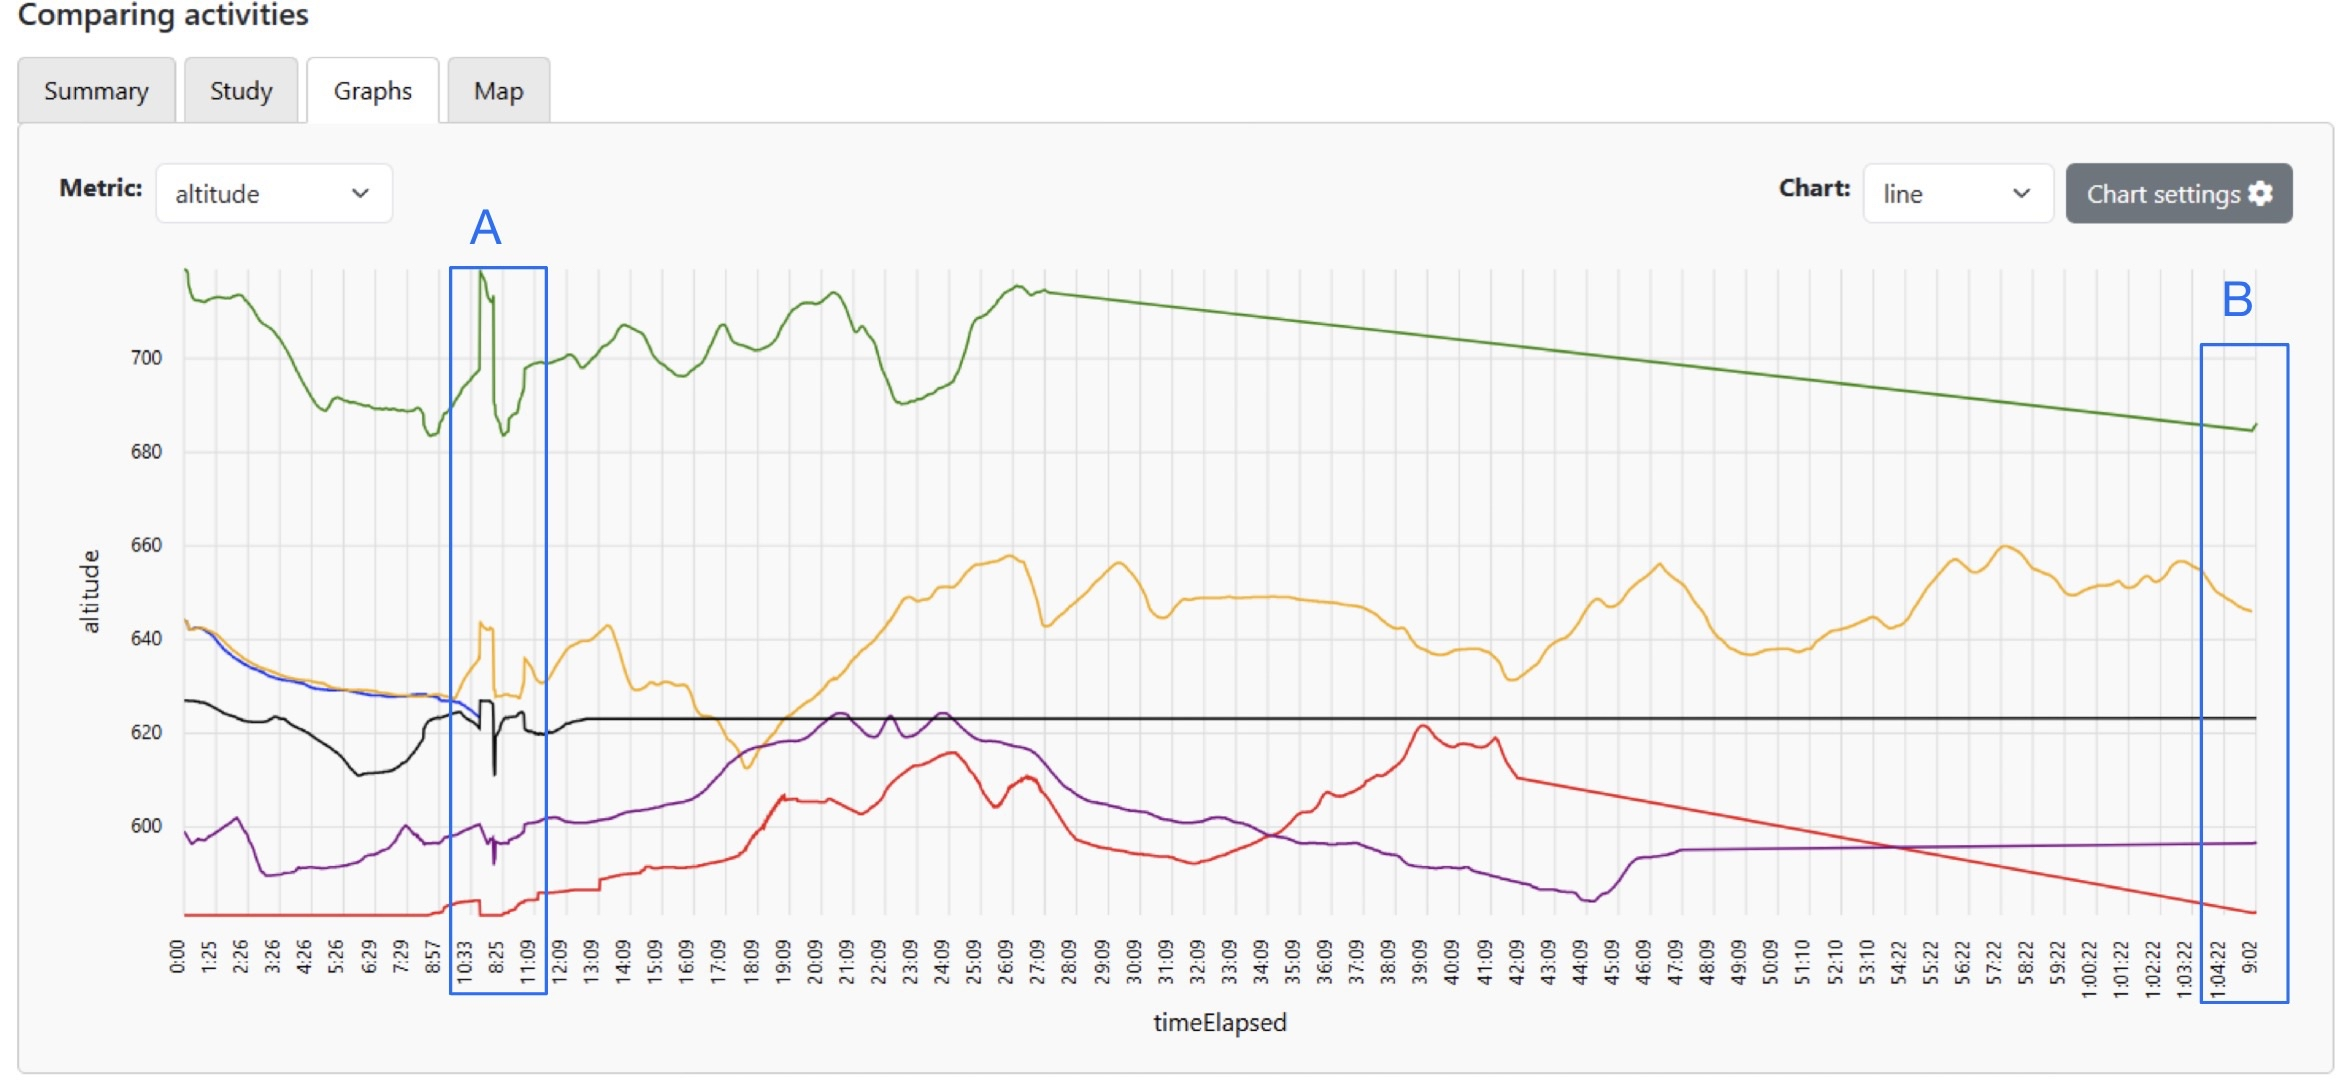
\includegraphics[width=0.75\linewidth]{img/ngx_algo_bad.png}
    \caption{Imagen ilustrativa del funcionamiento por defecto de ngx-charts}
    \label{fig:ngx_algo_bad}
\end{figure}

Hay dos principales puntos de interés, marcados como A y B. En el punto A se observa, en los valores del eje \texttt{x}, que pasa de 10:03 a 8:25, y luego de nuevo a 11:09. Este salto se ve reflejado también en los valores de las gráficas, que dan un salto sustancial en estos puntos. Además, este punto es donde acaba la actividad más corta (azul), lo cual parece causar la discrepancia. También podemos observar que varias de las series tienen un comportamiento extraño, dibujando una línea recta entre un punto arbitrario de la gráfica hasta la sección B. Las más notables son las series negra y verde, pero se presenta también en la roja y la morada. El error aquí es similar. Unos pocos valores de todas estas gráficas están siendo mostrados después de que termine la gráfica amarilla. Se puede ver también en el eje \texttt{x} que los valores pasan de 1:04:22 a 9:02. Presumiblemente la serie amarilla no tiene valores de \texttt{y} para las \texttt{x} alrededor de 9:02, y está siendo priorizada sobre las otras, por lo que estos valores se muestran después de que acabe.

Como se puede ver, no es un comportamiento intuitivo, y rompe completamente la visualización de las gráficas, causando saltos arbitrarios y líneas innecesarias. Por esto ha sido necesario implementar esta solución, tras la cual esa misma gráfica se muestra como se ve en la figura \ref{fig:ngx_algo_good}
\begin{figure}[H]
    \centering
    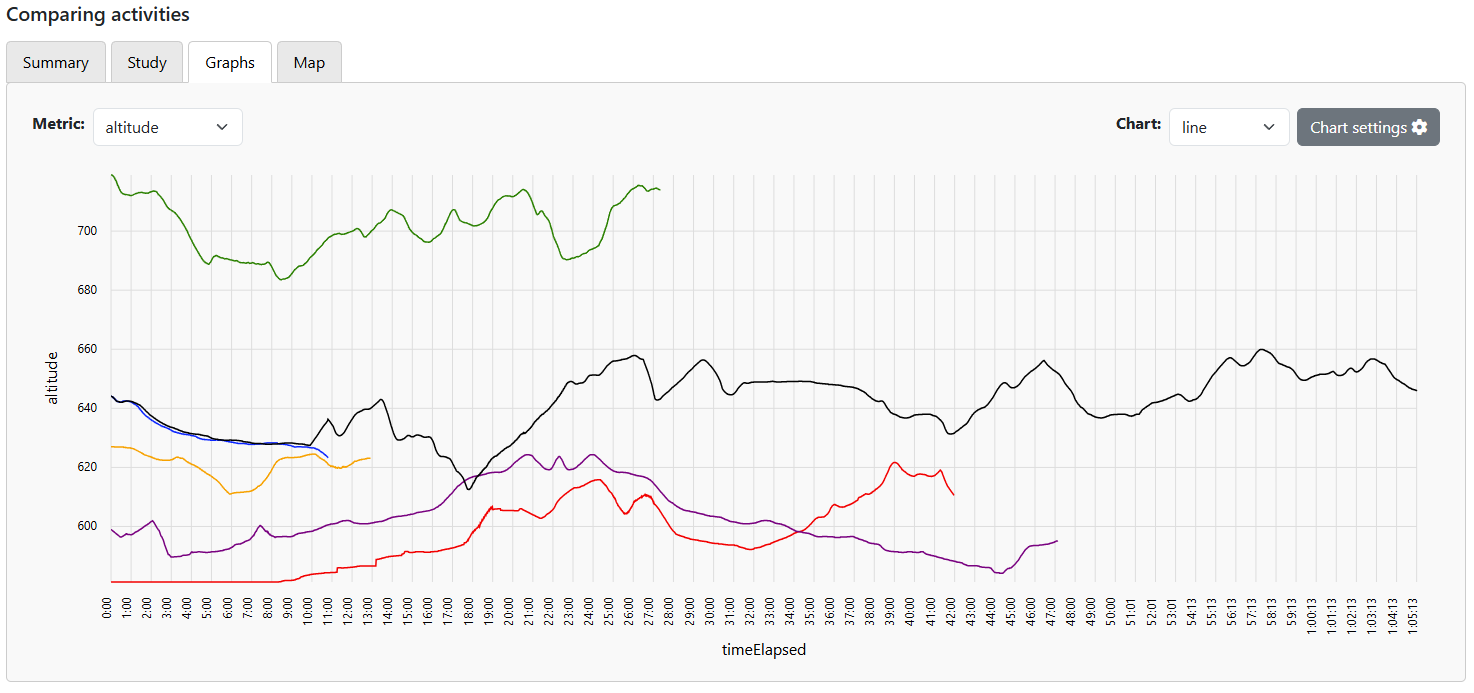
\includegraphics[width=0.75\linewidth]{img/ngx_algo_good.png}
    \caption{Imagen ilustrativa del funcionamiento de ngx-charts aplicando el algoritmo de interpolación}
    \label{fig:ngx_algo_good}
\end{figure}
En esta figura se puede ver que cada serie acaba cuando debe, sin dar saltos arbitrarios ni alargarse más de lo necesario, y leyendo los valores del eje \texttt{x} se puede confirmar que están todos ordenados correctamente.

\subsection{Cálculo de récords}
Una de las herramientas que se ha decidido incluir en la aplicación es el cálculo de récords, para que los usuarios puedan tener un registro de sus mejores marcas en distintas métricas a lo largo del tiempo y saber cuándo superan marcas concretas. Se consideran dos tipos de récords: récords de distancia, y récords de tiempo. Miden el mínimo tiempo tomado para cubrir una distancia fija, y la máxima distancia cubierta en un tiempo fijo, respectivamente.

Se incluyen en esta sección debido a que la forma de calcularlos se ha considerado de interés. Se utiliza un algoritmo ligeramente distinto para cada tipo de récord, aunque tienen puntos en común. La idea de ambos es utilizar una ventana deslizante para encontrar todos los tramos de tiempo o distancia especificados y quedarse con el que mejor marca tenga. A continuación se muestra el código responsable de calcular los récords de distancia.


\begin{lstlisting}[ caption={Algoritmo de cálculo de récords de distancia}, label={lst:rest}]
private Long distanceGoal(List<String> positionStream, List<String> timeStream, int goal) {
        //preprocess streams
        List<Double[]> latlon = parseLatLon(positionStream);
        List<Double> segmentDistances = calcSegmentDistances(latlon);
        List<Instant> times = timeStream.stream().map(Instant::parse).toList();

        int i = 0;
        long bestTime = Long.MAX_VALUE ; //seconds
        double accumulatedDistance = 0; //meters
        for (int j = 1; j < latlon.size(); j++) {
            accumulatedDistance += segmentDistances.get(j-1);
            while (accumulatedDistance>=goal) {
                Instant i1 = times.get(i);
                Instant i2 = times.get(j);

                long currentTime = Duration.between(i1, i2).getSeconds();
                bestTime = Math.min(bestTime, currentTime);

                if (i + 1 >= j) break;
                accumulatedDistance -= segmentDistances.get(i);
                i++;
            }
        }
        return bestTime==Long.MAX_VALUE ? -1:bestTime; //seconds
    }
\end{lstlisting}

Para que el bucle sea lo más eficiente posible, se empieza transformando las posiciones, recibidas como \texttt{String} a \texttt{Double} en el \textit{array} \texttt{latlon}, y calculando las distancias entre cada posición, para no calcularlas por duplicado en el bucle. Luego, se hace lo mismo para los tiempos, transformándolos de \texttt{String} a \texttt{Instant}, de forma que puedan ser usados en el bucle sin tener que transformarlos varias veces.

Mediante el bucle \textit{for} se aumenta en uno la posición final de la ventana, y en el bucle \textit{while} se comprueba si la nueva distancia sobrepasa la distancia objetivo. En caso negativo se continúa hasta que se sobrepase, en cual momento se usará el bucle \textit{while} para aumentar el inicio de la ventana hasta que la distancia entre el inicio y el final sea menor al objetivo. Es importante que sea un bucle \textit{while} y no una condición simple debido a la irregularidad de los datos.

Pongamos por ejemplo queremos encontrar el récord de menor tiempo en cubrir 1km. Supongamos que los 9 primeros puntos están a intervalos regulares de 0.1km, pero el décimo punto, debido a una desconexión, está a 0.5km de distancia del noveno. El algoritmo inicialmente identificará una distancia de 1.4km, entre el punto inicial y el punto 10. Reconocerá que es mayor que 1km, así que guardará el tiempo tomado en \texttt{bestTime}. Si no se incluyera el bucle \textit{while}, avanzaría el índice inicial una posición, y continuaría moviendo el final de la ventana, aunque la distancia acumulada actualmente es 1.3km, y el tiempo será mejor. Incluyendo el bucle, aseguramos que no continúe moviendo el final de la ventana hasta que la distancia acumulada sea menor al objetivo, asegurando así que la marca almacenada en \texttt{bestTime} se ajuste lo mejor posible a la realidad. La tabla \ref{tab:sliding_window} muestra el funcionamiento del algoritmo en este caso
\begin{table}[h!]
    \centering
    \begin{tabular}{|c|c|c|c|c|}
        \hline
        Iteración & $p_i$ & $p_f$ & Distancia (km) & BestTime (s) \\ \hline
        1  & 0 & 0  & 0.0  & $\infty$ \\ \hline
        2  & 0 & 1  & 0.1  & $\infty$ \\ \hline
        3  & 0 & 2  & 0.2  & $\infty$ \\ \hline
        \vdots & \vdots & \vdots & \vdots & \vdots \\ \hline
        8  & 0 & 8  & 0.8  & $\infty$ \\ \hline
        9  & 0 & 9  & 0.9  & $\infty$ \\ \hline
        10 & 0 & 10 & 1.4  & 380 \\ \hline
        11 & 1 & 10 & 1.3  & 370 \\ \hline
        12 & 2 & 10 & 1.2  & 360 \\ \hline
        13 & 3 & 10 & 1.1  & 350 \\ \hline
        14 & 4 & 10 & 1.0  & 340 \\ \hline
        15 & 5 & 10 & 0.9  & 340 \\ \hline
        16 & 5 & 11 & 1.0  & 340 \\ \hline
        \end{tabular}
        \caption{Funcionamiento del algoritmo de ventana deslizante ante irregularidades en los datos.}
        \label{tab:sliding_window}
\end{table}

Este bucle tiene el potencial de introducir un error. Si por cualquier razón el intervalo entre dos puntos fuera mayor al objetivo, podría seguir incrementando el inicio de la ventana más allá del final de esta. Para evitarlo, se ha incluido un break para asegurar que, si el inicio y final de la ventana son consecutivos, deje de incrementar el inicio de la ventana.

\section{Control de calidad} 
Todo proyecto de software debe tener herramientas de control de calidad para asegurar que el código desarrollado, así como el que se desarrolle a futuro, sea de calidad, no introduzca errores, ni incremente excesivamente la complejidad del sistema.

En este proyecto se han implementado dos medidas para garantizar la calidad del código: pruebas que evalúan dinámicamente el código, ejecutándolo y comprobando su correcto funcionamiento, y análisis estático de código, utilizando herramientas que analizan el código sin ejecutarlo para identificar potenciales vulnerabilidades, problemas de complejidad, malos olores, y otros defectos potenciales.

Se han implementado pruebas dinámicas de tres tipos: unitarias, de integración, y de extremo a extremo. Las pruebas unitarias son las más extensas. Comprueban el correcto funcionamiento de métodos y clases concretas, probando todos los posibles caminos, considerando errores y distintos parámetros. Las pruebas de integración comprueban que los distintos componentes se comuniquen entre sí correctamente y funcionen bien en conjunto. En este proyecto concretamente, se han utilizado para comprobar la conexión con la base de datos y asegurar que las peticiones personalizadas a la base de datos funcionen correctamente. Por último están las pruebas de extremo a extremo, o end to end, abreviadas e2e. Estas comprueban el comportamiento completo de la aplicación, simulando las acciones de un usuario. No se centran en probar el correcto funcionamiento de componentes concretos, sino que simulan distintos flujos que podría realizar un usuario, y comprueban que todo funciona como es debido. Pueden evaluar casos correctos, referidos como \textit{happy path}, o casos incorrectos, donde comprueba que al intentar realizar acciones no permitidas la aplicación lanza las excepciones esperadas. 

\subsection{Pruebas unitarias}
Se han desarrollado 188 pruebas unitarias, centradas principalmente en los servicios. De cada servicio se han identificado los métodos más importantes, los que se usan con más frecuencia, o los que son más complejos, y se han implementado pruebas para todos los posibles caminos del código en ese método. La cobertura de código por servicio es:
\begin{table}[H]
\centering
\begin{tabular}{l c}
\hline
\textbf{Servicio} & \textbf{Cobertura} \\
\hline
ActivityService & 52.9\% \\
RouteService    & 75.9\% \\
MuralService    & 85.8\% \\
UserService     & 85.1\% \\
\hline
\end{tabular}
\caption{Porcentaje de cobertura por servicio}
\label{tab:cobertura-servicios}
\end{table}
ActivityService tiene una cobertura menor dado a que es el servicio más grande. Por tanto, aunque se han cubierto un número similar de funcionalidades que en los otros servicios, al tener más funcionalidades en total, la cobertura resultante es más baja.

Los métodos probados explícitamente mediante pruebas unitarias se detallan en la tabla \ref{pruebas_unitarias}:
\begin{table}[H]
\small
\centering
\renewcommand{\arraystretch}{0.85} % Mantiene el interlineado compacto
\begin{tabularx}{\textwidth}{@{} l X @{}}
\toprule
\textbf{Servicio} & \textbf{Métodos cubiertos por pruebas unitarias} \\ \midrule
\textbf{ActivityService} & Cambiar visibilidad, Borrar ruta, Obtener actividad por ID, Fijar ruta, Borrar actividad, Editar actividad. \\ \addlinespace
\textbf{MuralService} & Crear mural, Unirse a mural, Banear usuario, Borrar a usuario de mural, Desbanear usuario, Borrar mural, Editar mural. \\ \addlinespace
\textbf{RouteService} & Cambiar visibilidad, Obtener actividades en la ruta, Obtener listado de todas las rutas, Crear ruta, Añadir actividades a ruta, Borrar ruta. \\ \addlinespace
\textbf{UserService} & Crear usuario, Modificar usuario, Borrar usuario. \\ \bottomrule
\end{tabularx}
\caption{Funcionalidades cubiertas por pruebas unitarias}
\label{pruebas_unitarias}
\end{table}
Se ha procurado seleccionar las funcionalidades principales de cada entidad, o aquellas que son esenciales para su correcto funcionamiento, haciendo énfasis en la creación y eliminación de entidades. Además, para las Actividades y Rutas, se ha probado la lógica de cambiar visibilidad, ya que se considera especialmente compleja. Destaca la falta de pruebas de creación de actividad. Esto se debe al hecho de que las actividades se crean a partir de archivos, lo cual dificulta su comprobación en pruebas unitarias. Se ha preferido cubrir ese caso con las pruebas e2e.

\subsection{Pruebas de Integración}
Dada la relativa sencillez del despliegue de la aplicación, no se ha considerado necesario desarrollar una amplia suite de pruebas de integración, dado que no depende de APIs externas ni otros servicios similares. Por tanto, se ha decidido focalizar las pruebas de integración en la conexión con la base de datos, ya que la correcta comunicación entre servidor y cliente se probará como parte de las pruebas e2e.

Se ha creado una prueba de integración para cada consulta personalizada a la base de datos. Esto ha resultado en 10 pruebas distintas divididas entre dos clases. Estas consultas, con carácter general, devuelven una serie de registros que cumplen unas características definidas, como pertenecer a un usuario concreto, tener un valor específico en un campo concreto, etcétera.

\subsection{Pruebas de Extremo a Extremo}
Al contrario que en el resto de pruebas, las pruebas de extremo a extremo (e2e) no prueban funcionalidades únicas, sino que evalúan secciones de la aplicación al completo, trabajando habitualmente en flujos. Por ejemplo, un flujo básico podría ser iniciar sesión, navegar a la sección de creación de una entidad, crear la entidad, y verificar los datos de la entidad creada. Dado este cambio en el enfoque, y que prueban tanto cliente como servidor, son las más costosas de implementar, además de ser de las pruebas más frágiles; un simple cambio en la interfaz puede romperlas. Por tanto, no es aconsejable definir pruebas e2e para todas las funcionalidades, sino que se prefiere limitarse a los flujos esenciales de la aplicación. En este caso, se han implementado 9 flujos, probando la creación y eliminación de las distintas entidades, junto con alguna prueba adicional:
\begin{multicols}{2}
\begin{enumerate}
    \item Comprobar info. usuario 
    \item Crear Actividad
    \item Seleccionar Actividad
    \item Borrar Actividad
    \item Crear Ruta
    \item Borrar Ruta
    \item Crear Mural
    \item Seleccionar Mural
    \item Borrar Mural
\end{enumerate}
\end{multicols}

\subsection{Análisis estático de código}
Además del análisis dinámico de código mediante pruebas, se ha realizado un control de calidad mediante análisis estático de código utilizando SonarQube.

Al analizar el código con SonarQube, la herramienta ofrece el siguiente resumen:
\begin{figure}[H]
    \centering
    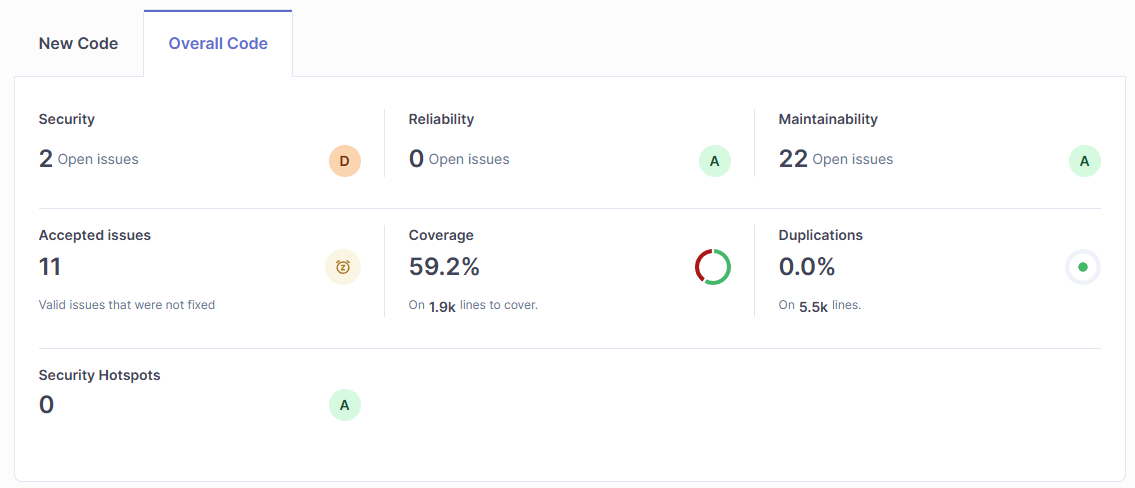
\includegraphics[width=0.75\linewidth]{img/analisis_sonarqube.png}
    \caption{Resumen del análisis realizado por SonarQube}
    \label{fig:analisis_sonarqube}
\end{figure}
A través de los resúmenes de SonarQube se ha llevado a cabo un proceso de optimización y refactorización para mejorar la calidad del código, eliminando muchos de los \textit{issues} que lanza. Concretamente, la herramienta había identificado varios problemas de fiabilidad y mantenibilidad que han sido tenidos en cuenta durante las últimas fases del desarrollo. La figura \ref{fig:analisis_sonarqube} muestra los resultados  de SonarQube una vez solucionados estos problemas. 

Se puede ver que hay 2 \textit{Open issues} en \textit{Security}, 22 en \textit{Maintainability}, y 11 \textit{Accepted issues}. Estos \textit{issues} no han sido corregidos ya que, o bien se ha juzgado que no son problemas reales para la aplicación en su estado y alcance actual, o bien se considera que el coste de arreglarlos en este momento es mayor que el beneficio de haberlos arreglado. Dicho esto, entremos en más detalle sobre cada sección y por qué se considera aceptable:

\subsubsection{Security}
Los dos \textit{issues} en \textit{security} son por usar un modo de cifrado no seguro, concretamente \texttt{"AES/ECB/PKCS5Padding"}. El problema viene con el modo ECB (\textit{Electronic CodeBook)}, ya que cifra bloques iguales en textos iguales y filtra patrones del texto original (entre otras vulnerabilidades), lo que permite a potenciales atacantes detectar partes repetidas, reconstruir la estructura de los datos, e identificar campos iguales. Una alternativa posible sería usar  \texttt{"AES/GCM/NoPadding"}, que soluciona estos problemas. Sin embargo, cambiar a usar este cifrado requiere cambiar código sensible que gestiona autenticación y seguridad, que fue tomado de un proyecto de referencia proporcionado por los profesores. Dada la sensibilidad del código, la poca familiaridad del autor con él, la gravedad de las consecuencias de cometer errores durante el supuesto \textit{fix}, y el relativo bajo impacto de la vulnerabilidad para la aplicación en su estado actual, se ha decidido aceptar el riesgo planteado por esta vulnerabilidad. Sin embargo, es una vulnerabilidad real, y según la aplicación crezca será necesario solucionarla.

\subsubsection{Accepted Issues}
Hay 11 \textit{issues} marcados como aceptados. Los 11  indican que las contraseñas usadas en la inicialización de la base de datos están comprometidas y deben ser modificadas. Dado que estos datos son de ejemplo y las contraseñas no pretenden ser seguras, no se considera que estas vulnerabilidades tengan un efecto real sobre la aplicación ni que necesiten ser solucionadas. Por tanto, han sido marcadas como aceptadas.


\subsubsection{Maintainability}
Hay 22 \textit{issues} de mantenibilidad. De estos, la mayoría son menores, y se ha decidido no solucionarlos porque tienen poco efecto real, por dejar espacio de ampliación, o porque se considera que solucionarlos conlleva un esfuerzo innecesario comparado con el beneficio de solucionar el problema. Los más graves son 4 instancias de métodos con complejidad cognitiva demasiado alta. Estos \textit{issues} plantean preocupaciones más graves, recalcando una serie de métodos que, como indica el análisis, son difíciles de entender y seguir. En este caso, no se han solucionado porque la dificultad de solucionarlos y el tiempo requerido para ello se considera mayor que el beneficio que aporta simplificar los métodos para la aplicación en su estado actual. Sin embargo, es una preocupación real, que deberá ser tratada según la aplicación crezca. 

\section{Despliegue}
El empaquetado y despliegue de la aplicación es una fase importante en todo proyecto, pues es el proceso a través del cual la aplicación y los nuevos cambios se hacen accesibles a los usuarios. Es importante que sea un proceso estable y reproducible, pues a lo largo del desarrollo de una aplicación se puede esperar realizar despliegues con relativa frecuencia. Para garantizar esta reproducibilidad el despliegue se suele hacer de manera automatizada mediante pipelines y workflows.

Esta sección documenta cómo es cada parte del proceso de despliegue de la aplicación. Se ha dividido en tres subsecciones:
\begin{enumerate}
    \item \textbf{Empaquetado:} proceso según el cual se generan artefactos a partir del código
    \item \textbf{Distribución:} detalla dónde y cómo estos artefactos son almacenados, así como la forma de acceder a ellos 
    \item \textbf{Despliege:} proceso según el cual el código es puesto en ejecución de manera que sea accesible para los usuarios  
\end{enumerate}

\subsection{Empaquetado}
Se ha utilizado Docker como herramienta para el empaquetado de la aplicación y la generación de artefactos. Dado que la parte cliente y la parte servidor son independientes, se empaquetan en artefactos independientes. Por tanto, se han redactado dos archivos Dockerfile que configuran cómo debe ser creado cada uno de estos artefactos. Para la ejecución en local de la aplicación a partir de estos artefactos, se ha configurado un Docker Compose, encargado de orquestar estas dos imágenes, junto con una imagen adicional para la base de datos. Sin embargo, para la ejecución en el entorno de despliegue/producción, esta configuración no es viable porque Azure Container Instances no soporta docker-compose directamente.

Para la ejecución en producción los artefactos se ejecutan en contenedores públicos, disponibles desde URLs públicas. Por tanto, simplemente se han configurado las imágenes y el código para que, en vez de comunicarse a través de una red común configurada en el Docker Compose, se comuniquen directamente a través de estas URLs públicas.

\subsection{Distribución}
Las imágenes se pueden generar manualmente, aunque por norma general serán generadas de manera automática por workflows de GitHub Actions cada vez que se suban cambios a la rama main. Estos workflows generan las imágenes siguiendo la configuración definida en cada Dockerfile, y las suben a DockerHub,  desde donde quedan disponibles públicamente. Concretamente, se publican bajo el usuario \href{https://hub.docker.com/u/angelmarquesgarcia}{\uline{angelmarquesgarcia}\footnote{\url{https://hub.docker.com/u/angelmarquesgarcia}}}. Las imágenes del cliente se publican en el repositorio 
\href{https://hub.docker.com/r/angelmarquesgarcia/atra-frontend}{\uline{angelmarquesgarcia/atra-frontend}\footnote{\url{https://hub.docker.com/r/angelmarquesgarcia/atra-frontend}}}, mientras que las del servidor son accesibles en el repositorio
\href{https://hub.docker.com/r/angelmarquesgarcia/atra-backend}{\uline{angelmarquesgarcia/atra-backend}\footnote{\url{https://hub.docker.com/r/angelmarquesgarcia/atra-backend}}}.


\subsection{Despliegue}

El despliegue se realiza en Azure. Concretamente, cada parte de la aplicación (cliente y servidor) se despliega en un contenedor de Azure, dentro de un Azure Resource Group común. Además, en ese mismo resource group hay una instancia de Azure Database for MySQL flexible server, que se ocupa de la gestión de la base de datos.

\begin{figure}[H]
    \centering
    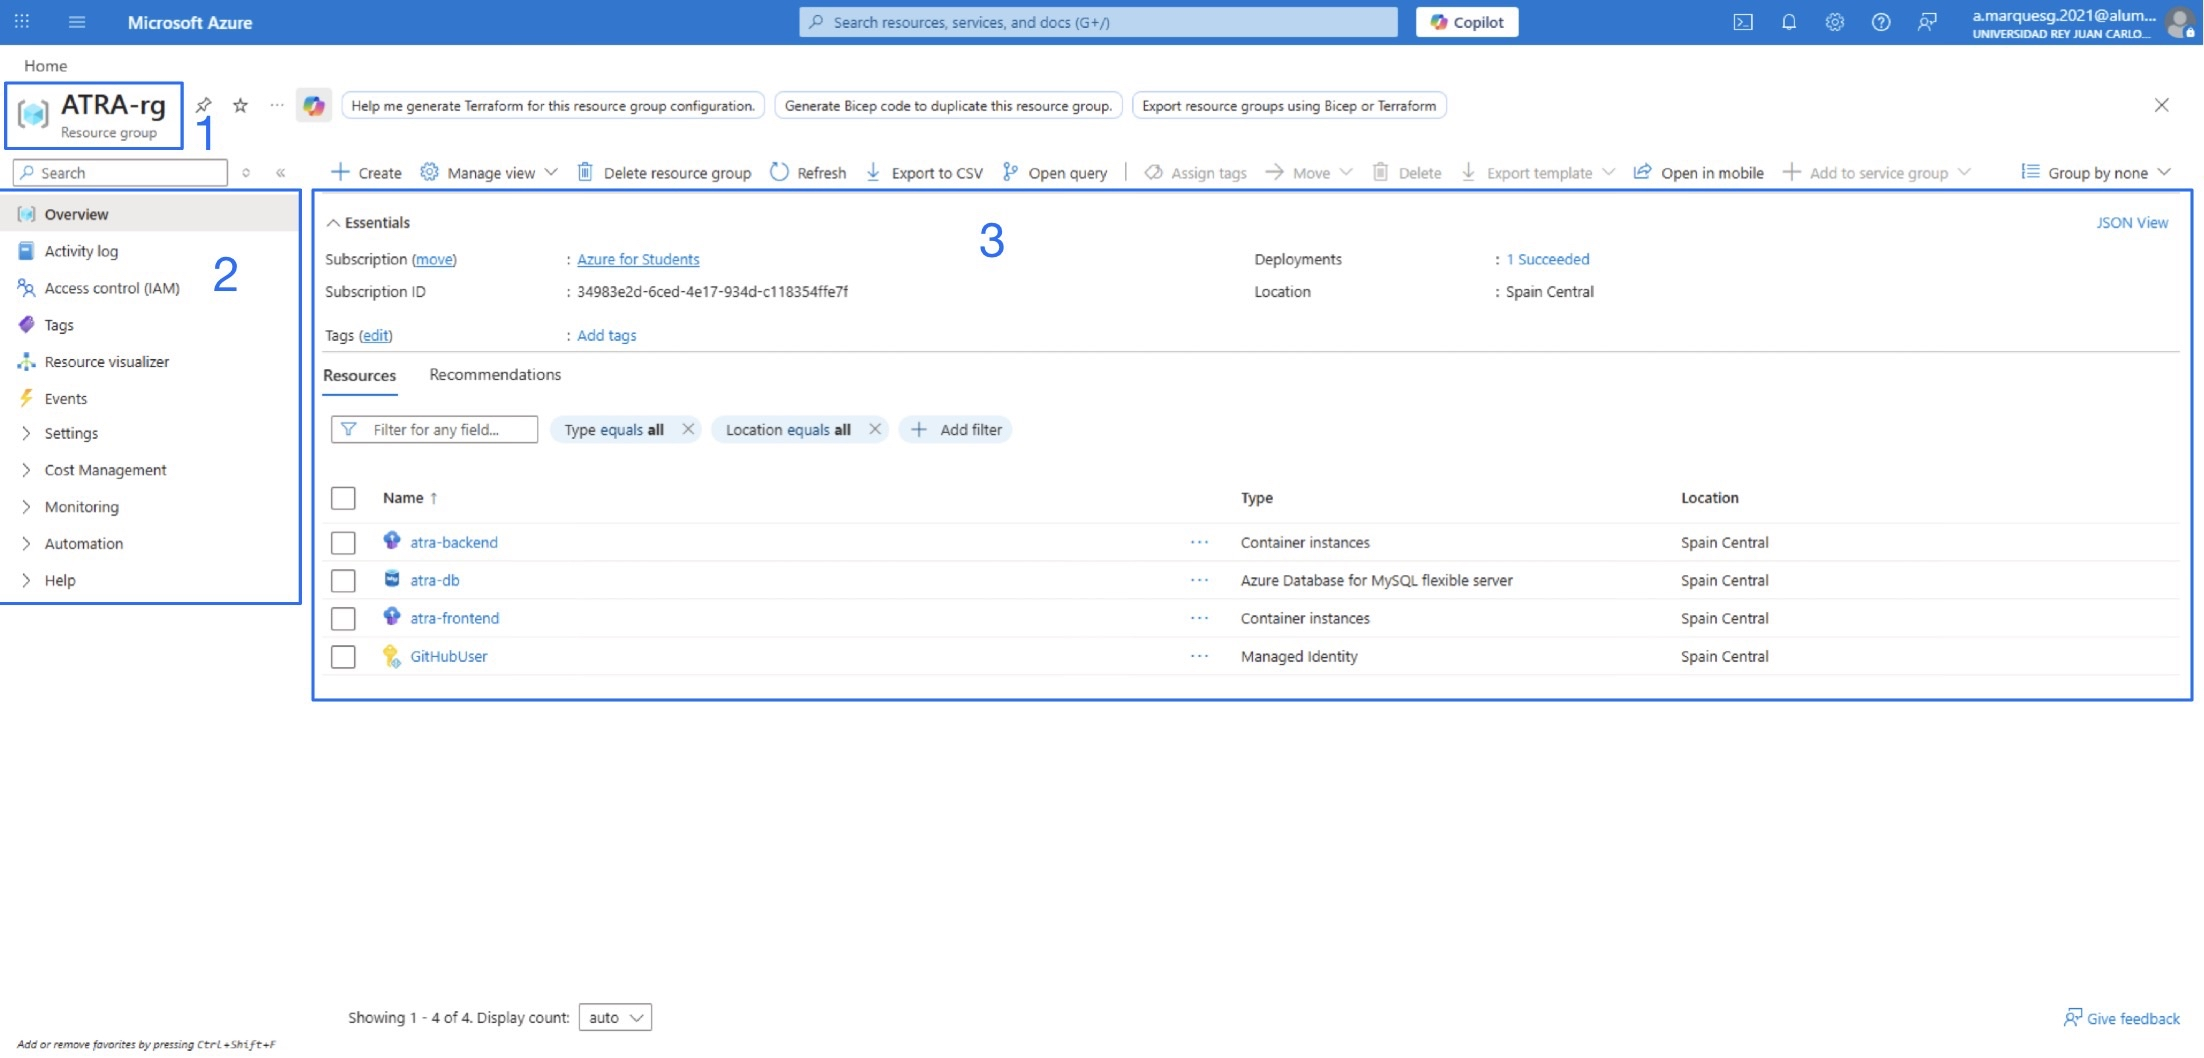
\includegraphics[width=1\linewidth]{img/azure_dashboard.png}
    \caption{Panel de Control de Azure}
    \label{fig:azure_dashboard}
\end{figure}

En la figura \ref{fig:azure_dashboard} se puede ver el panel de control de Azure, mostrando los recursos creados. En la sección 1 se puede ver el \textit{resource group}, denominado "ATRA-rg". En Azure, los \textit{resource groups} son elementos que permiten agrupar otros elementos en un espacio común, de forma que se facilite la gestión de los distintos recursos de Azure. Para este proyecto, sólo ha sido necesario definir este \textit{resource group}.

La sección 2 es un menú lateral que permite navegar por las distintas secciones y herramientas de Azure, para gestionar distintas características y propiedades del \textit{resource group}. Está seleccionado el \textit{overview}, que ofrece una visión general del producto y los recursos incluidos en él.

La sección 3 muestra la herramienta seleccionada en el menú lateral, en este caso un \textit{overview} de las características y elementos principales en el \textit{resource group}. En la mitad superior podemos ver información sobre el \textit{resource group}, como la suscripción bajo la que se incluye o la localización en la que se ubica. En la parte inferior, podemos ver una lista con los distintos recursos de Azure incluidos en este \textit{resource group}. Podemos ver que hay dos \textit{Container instances}, un \textit{Azure Database for MySQL flexible server}, y una \textit{Managed Identity}, y que todas se ubican, al igual que el \textit{resource group}, en los servidores de Azure en España Central. A continuación describiremos un poco más a fondo qué es cada uno de estos recursos \cite{azure}.

\begin{itemize}
    \item \textbf{Container Instances}: un servicio serverless que permite ejecutar imágenes de Docker sin tener que gestionar la infraestructura subyacente. Al crear el recurso, se le proporciona una imagen de Docker, y simplemente la ejecuta. En este proyecto se ha usado para desplegar de manera independiente el \textit{frontend} y el \textit{backend} a partir de las imágenes publicadas en DockerHub.
    \item \textbf{Azure Database for MySQL flexible server}: un servicio administrado de bases de datos MySQL en Azure. El hecho de que sea administrado significa que Azure es responsable de gestionar la infraestructura, copias de seguridad, parches, y demás, mientras que el desarrollador sólo se tiene que preocupar de gestionar y configurar la base de datos en sí, los \textit{Schemas}, usuarios, etc. En este proyecto se usa como la base de datos en producción del sistema.
    \item \textbf{Managed Identity:} es una identidad gestionada por azure, que permite a un recurso (en este caso el agente de GitHub Actions), autenticarse en Azure para realizar operaciones sin tener que almacenar credenciales o datos sensibles en el código.
\end{itemize}

\subsubsection{Flujo de despliegue}
Los componentes (cliente y servidor) son actualizados de manera independiente cada vez que se hace push con cambios a la parte correspondiente. Es decir, si se introducen cambios al cliente, se actualiza el contenedor del cliente, pero no el del servidor, y viceversa.

Más en detalle, el flujo de despliegue consiste en dos workflows de GitHub Actions, uno para cambios a la \href{https://github.com/codeurjc-students/2024-Atra/blob/main/.github/workflows/build_and_deploy_frontend.yml}{\uline{parte cliente}\footnote{\url{https://github.com/codeurjc-students/2024-Atra/blob/main/.github/workflows/build_and_deploy_frontend.yml}}}, y otro para cambios a la \href{https://github.com/codeurjc-students/2024-Atra/blob/main/.github/workflows/build_and_deploy_backend.yml}{\uline{parte servidor}\footnote{\url{https://github.com/codeurjc-students/2024-Atra/blob/main/.github/workflows/build_and_deploy_backend.yml}}}. Estos workflows son disparados cuando se hace un push a main con cambios a las respectivas partes, y ejecutan dos tareas:
\begin{enumerate}
    \item \textbf{build:} compilan la parte de la aplicación correspondiente, la empaquetan en una imagen de Docker, y suben esta imagen a DockerHub 
    \item \textbf{deploy:} inicia sesión en Azure, y crea un contenedor desde el que ejecutar la imagen creada en el paso build.
\end{enumerate}
Adicionalmente, en el caso del workflow de \textit{backend}, debe ejecutar un paso adicional, que consiste en reiniciar el contenedor en el que se ejecuta el \textit{frontend}. Esto es necesario para actualizar la dirección a la que apunta el \textit{proxy} del \textit{frontend}.

Como nota final, para la comunicación entre los contenedores y con la base de datos, es necesario establecer variables de entorno. Estas se incluyen en el comando utilizado para actualizar los contenedores (dentro de la tarea \textit{deploy}), de forma que: 1. El código puede acceder a ellas, y 2. se pueden almacenar de manera segura como secretos de GitHub.

\section{Proceso de desarrollo} 
La gestión de tareas se refiere al uso de herramientas de gestión que permiten llevar un seguimiento de las distintas tareas que es necesario completar durante el desarrollo del proyecto, permitiendo visualizar, cuanto menos, tareas pendientes, tareas en progreso, y tareas completadas.

Es importante en todo proyecto mantener una gestión de tareas adecuada, para evitar que haya funcionalidades que queden olvidadas, problemas que se queden sin resolución, etc. Además, una buena gestión de tareas permite la división de tareas y responsabilidades en proyectos más grandes, facilitando la colaboración. Incluso en proyectos pequeños, ayuda ofreciendo una visión más general del trabajo pendiente y en progreso, asegurando que los desarrolladores mantengan una visión global del proyecto y de cómo su trabajo encaja en el mismo, y permitiendo el control del trabajo en progreso, para evitar casos en los que se intenta afrontar demasiadas tareas simultáneamente y no avanza ninguna, o algunas quedan olvidadas.

Debido al reducido alcance de este proyecto (un único desarrollador, no hay necesidad de coordinar tareas), no se ha considerado necesario utilizar a fondo herramientas de gestión de tareas. Sin embargo, esto no quiere decir que no haya habido gestión de tareas. Desde la primera fase de definición de funcionalidades, se han tomado las funcionalidades descritas como la lista de tareas pendientes, y se ha establecido un orden y prioridad para su desarrollo. Luego, durante el desarrollo, los errores y problemas encontrados se han ido apuntando en una lista aparte, inicialmente a través de GitHub Issues. Sin embargo, por conveniencia, ha resultado más fácil mantener una lista organizada en un documento de texto, pues resulta más fácil de gestionar. Si bien no ha habido una lista de tareas en progreso tradicional, tampoco ha resultado muy necesaria, pues, salvo contadas excepciones, sólo se ha trabajado en una tarea a la vez.

\subsection{Git} 
Git es una herramienta esencial en todo proyecto de software, ya que ofrece un sistema para el versionado, colaboración, control de cambios, etc, ofreciendo trazabilidad total de todas las operaciones,  y facilitando \textit{rollback} (volver a una versión anterior). Incluso en proyectos pequeños, la capacidad de controlar los cambios, ver el historial de los mismos, y mantener una copia de seguridad del software desarrollado en todo momento hace de Git una herramienta de uso imperativo.

Git puede ser utilizado individualmente como una herramienta independiente. Sin embargo, por norma general, se utiliza a través de algún otro servicio, como GitHub o GitLab, que permite una gestión de las operaciones más sencilla, ofrece interfaces visuales, y ofrece otras herramientas adicionales. Para este proyecto se ha decidido usar GitHub como \textit{host} para el repositorio. Concretamente, se ha creado un repositorio público accesible en \href{https://github.com/codeurjc-students/2024-Atra}{este enlace}\footnote{\url{https://github.com/codeurjc-students/2024-Atra}}

El uso de Git ha sido constante durante todo el proceso de desarrollo, acumulando un total aproximado de 300 commits en 3 ramas. La mayoría de los commits son directos sobre la rama main, ya que es donde se han desarrollado la mayoría de funcionalidades, habiendo sido creadas las otras dos ramas para realizar pruebas varias de CI/CD, y para el desarrollo de una página concreta. Adicionalmente, existe una rama adicional que se ha mantenido en local cuya función fue permitir probar ciertas funcionalidades sin necesidad de modificar la rama principal.

Para que el historial de commits del repositorio sea fácil de leer y se pueda conocer los cambios incluidos en un commit sin mirar el código, se ha seguido el estándar de nomenclatura \href{https://www.conventionalcommits.org/en/v1.0.0/}{\uline{Conventional Commits}\footnote{\url{https://www.conventionalcommits.org/en/v1.0.0/}}}, junto con mensajes clarificativos en la descripción cuando se ha considerado necesario. 

\subsection{Integración y entrega continua} 
Para garantizar la integración continua y poder hacer entregas frecuentes de manera automática se han configurado una serie de workflows en GitHub actions. En esta sección se detalla cada uno de estos workflows, junto con sus pasos. Los workflows están disponibles en el directorio \href{https://github.com/codeurjc-students/2024-Atra/tree/main/.github/workflows}{./github/workflows}\footnote{\url{https://github.com/codeurjc-students/2024-Atra/tree/main/.github/workflows}} desde la raíz del proyecto en GitHub. Adicionalmente, se proveerá un enlace al código fuente de cada workflow en su descripción.

\textbf{\href{https://github.com/codeurjc-students/2024-Atra/blob/main/.github/workflows/test_on_commit.yml}{\uline{Test on commit}\footnote{\url{https://github.com/codeurjc-students/2024-Atra/blob/main/.github/workflows/test_on_commit.yml}}}}

\noindent Es un workflow sencillo que se ejecuta cada vez que ocurre un commit sobre una rama que no sea main. Sólo tiene una tarea, que consiste en ejecutar las pruebas unitarias y de integración. Su función es permitir al autor del commit y a posibles supervisores conocer si el commit realizado rompe funcionalidad existente.

\newpage

\textbf{\href{https://github.com/codeurjc-students/2024-Atra/blob/main/.github/workflows/test_on_pull_request.yml}{\uline{Test on pull request}}} \footnote{\url{https://github.com/codeurjc-students/2024-Atra/blob/main/.github/workflows/test_on_pull_request.yml}}

Es un workflow sencillo que se ejecuta cada vez que se inicia un pull request hacia la rama main. Al igual que el anterior, sólo tiene una tarea, que consiste en ejecutar las pruebas unitarias, de integración, y e2e. Para poder ejecutar las pruebas e2e necesita que el cliente esté en ejecución. Por tanto debe ejecutarlo antes de realizar las pruebas. Estos son los pasos que sigue:

\begin{multicols}{2}
\begin{enumerate}
    \item Configura Java.
    \item Configura Node.
    \item Descarga dependencias del cliente.
    \item Compila la parte cliente.
    \item Ejecuta el cliente en 2º plano.
    \item Realiza pruebas unitarias, integración y e2e.
\end{enumerate}
\end{multicols}

Su función es permitir al autor del pull request y a su supervisor saber si el código que se va a portar a la rama main contiene errores o regresiones.

\textbf{\href{https://github.com/codeurjc-students/2024-Atra/blob/main/.github/workflows/build_and_deploy_backend.yml}{\uline{Build and deploy backend}\footnote{\url{https://github.com/codeurjc-students/2024-Atra/blob/main/.github/workflows/build_and_deploy_backend.yml}}}}

Es el workflow encargado de desplegar nuevas versiones del servidor a Azure. Se ejecuta cada vez que se ejecuta un push a main que contenga cambios en el código de la parte del servidor. Consiste en dos tareas: build y deploy.

Build es la tarea responsable de compilar el código, generar la imagen de Docker, y subirla a DockerHub para hacerla disponible. Para subir la imagen a DockerHub es necesario iniciar sesión, por lo que, para que funcione correctamente, se deberá incluir el nombre de usuario bajo el cual publicar la imagen en los secretos del repositorio de GitHub, así como un token que autorice al workflow a subir imágenes en su nombre. El workflow sigue los siguientes pasos:
\begin{enumerate}
    \item Configura Java.
    \item Crea una etiqueta para la imagen a partir de la versión especificada en el pom.xml.
    \item Genera la imagen de Docker utilizando el usuario y la etiqueta para nombrarlo.
    \item Inicia sesión en DockerHub con el usuario y el token.
    \item Sube la imagen generada a DockerHub.
\end{enumerate}

Deploy es la tarea responsable de desplegar la versión actualizada del código en Azure. Para ello, necesitará credenciales para iniciar sesión en Azure, que deberán estar almacenadas en los secretos del repositorio, así como la imagen subida durante el paso anterior. Sigue los siguientes pasos:
\begin{enumerate}
    \item Inicia sesión en Azure.
    \item Crea un contenedor en el que ejecutar la imagen.
    \item Inicia el contenedor.
    \item Reinicia el contenedor del cliente.
\end{enumerate}
El último paso es necesario para que el \textit{proxy} del cliente se actualice y apunte a la dirección IP del contenedor que acaba de ser creado, en vez de al contenedor anterior.

\textbf{\href{https://github.com/codeurjc-students/2024-Atra/blob/main/.github/workflows/build_and_deploy_frontend.yml}{\uline{Build and deploy frontend}\footnote{\url{https://github.com/codeurjc-students/2024-Atra/blob/main/.github/workflows/build_and_deploy_frontend.yml}}}}

Es el workflow encargado de desplegar nuevas versiones del cliente a Azure. Se ejecuta cada vez que se ejecuta un push a main que contenga cambios en el código de la parte del cliente. Al igual que el workflow "Build and deploy backend", consiste en dos tareas: build y deploy. Ambas tareas tienen las mismas responsabilidades que en el otro workflow, y siguen los mismos pasos, con una excepción. La tarea deploy en este workflow omite el paso de reiniciar el otro contenedor, pues es innecesario.


\subsection{Estrategia de ramas y commits}
Para que el repositorio del proyecto sea legible y se pueda utilizar al máximo, es importante seguir una estrategia de ramas y \textit{commits}, que estandarice la forma de trabajar sobre el repositorio. De esta manera es más fácil navegar por el historial de \textit{commits} y entender los cambios, y permite aprovechar al máximo las ventajas ofrecidas por la herramienta. Estas estrategias definen cuándo se deben crear ramas, cuándo y cómo estas se deben unir con la rama principal, qué pasos se deben tomar en ese proceso (automatizados o manuales), cómo se deben hacer los commits, y sobre qué ramas se pueden realizar, etc.

Para este proyecto se ha seguido una estrategia muy sencilla, dado que el alcance del proyecto (monorepo, un único desarrollador) no necesita de un control muy exacto de las operaciones. Se ha permitido hacer \textit{commit} sobre la rama principal libremente, y se han utilizado ramas para desarrollar alguna funcionalidad específica, así como para realizar distintas pruebas.

Esta estrategia se ha juzgado suficiente por la baja escala del proyecto. No es necesario coordinar varios equipos de desarrolladores, Quality Assurance, arquitectos, etc, la arquitectura es bastante sencilla, el desarrollo es lineal, desarrollando completamente una funcionalidad antes de pasar a la siguiente,  y la necesidad de realizar revisiones  o estudiar el historial es mínima. Por estas y otras razones, se ha considerado que utilizar una estrategia más compleja y restrictiva entorpecería el desarrollo en vez de facilitarlo, y se ha optado por seguir esta estrategia.

En lo que respecta a los despliegues, no se han realizado durante el desarrollo, sino que se ha realizado un despliegue  al final del desarrollo, una vez la aplicación ha llegado a su versión 1.0. En este momento es cuando se han configurado los workflows de CI/CD en GitHub Actions para realizar despliegues sucesivos cuando se incorporen cambios. La implementación de estos workflows para despliegues sucesivos necesita seguir un flujo de desarrollo más estricto, desarrollando las distintas funcionalidades en ramas distintas a main, y juntando los cambios de estas ramas con main cuando se quiera actualizar el despliegue, acción que también actualizará la versión de la aplicación. 

Se ha tomado la decisión de manejar los despliegues y los flujos de CI/CD al final del desarrollo ya que se ha preferido posponer el despliegue de la aplicación hasta que esta estuviera en un estado más o menos estable. En vez de desplegar la aplicación con funcionalidad parcial y actualizarla periódicamente con las distintas funcionalidades, se ha preferido centrar el esfuerzo completamente en el desarrollo para poder al final desplegar la aplicación al completo. Dado que no hay un cliente o una base de usuarios que necesiten acceso a la aplicación para verificar progreso, realizar pruebas, o ponerla en uso, se ha considerado adecuado limitar los despliegues de esta manera. Además, la puesta en despliegue de la aplicación y la gestión de los flujos de CI/CD utilizan tecnologías con las que el autor tiene poca familiaridad, por lo que se esperaba que fueran necesarios tiempos de familiarización y corrección de errores. Se ha preferido concentrar ese esfuerzo al final del proyecto, para que no interrumpa el desarrollo si, por ejemplo, fallara el despliegue de la aplicación tras la incorporación de una nueva funcionalidad.

